% Chapter 6: Model selection and risk management
% Statistics of Financial Markets -- Bachelor's programme, Bucharest University of Economic Studies
% GENERATED by latex/build_chapter6.py -- edit the generator, not this file.

\newcommand{\coursename}{Statistics of Financial Markets}
% Preambul comun SFM -- Statistica piețelor financiare / Statistics of Financial Markets (Beamer, 16:9)
% Același design ca MFM. Înainte de % Preambul comun SFM -- Statistica piețelor financiare / Statistics of Financial Markets (Beamer, 16:9)
% Același design ca MFM. Înainte de % Preambul comun SFM -- Statistica piețelor financiare / Statistics of Financial Markets (Beamer, 16:9)
% Același design ca MFM. Înainte de \input{../../latex/preamble} se definește
%   \newcommand{\coursename}{Statistics of Financial Markets}      (EN)
%   \newcommand{\coursename}{Statistica piețelor financiare}       (RO)  și  \def\sfmlang{ro}
% Fișierele .tex se află în EN/Courses, EN/Seminars, RO/Cursuri, RO/Seminarii (două niveluri sub rădăcină).
% Deck-urile sînt generate de latex/build_chapterN.py / build_seminarN.py (vezi latex/sfm_build.py).

\documentclass[9pt, aspectratio=169, t]{beamer}
\providecommand{\coursename}{Statistics of Financial Markets}

% Ensure content fits on slides
\setbeamersize{text margin left=8mm, text margin right=8mm}

%=============================================================================
% THEME AND STYLE CONFIGURATION
%=============================================================================
\usetheme{default}
% Using default theme for clean header/footer control

% Color Palette (matching Redispatch PDF)
\definecolor{MainBlue}{RGB}{26, 58, 110}
\definecolor{AccentBlue}{RGB}{26, 58, 110}
\definecolor{IDAred}{RGB}{205, 0, 0}
\definecolor{DarkGray}{RGB}{51, 51, 51}
\definecolor{MediumGray}{RGB}{128, 128, 128}
\definecolor{LightGray}{RGB}{248, 248, 248}
\definecolor{VeryLightGray}{RGB}{235, 235, 235}
\definecolor{KeynoteGray}{RGB}{218, 218, 218}
\definecolor{SectionGray}{RGB}{120, 120, 120}
\definecolor{FooterGray}{RGB}{100, 100, 100}
\definecolor{Crimson}{RGB}{220, 53, 69}
\definecolor{Forest}{RGB}{46, 125, 50}
\definecolor{Amber}{RGB}{181, 133, 63}
\definecolor{Orange}{RGB}{230, 126, 34}
\definecolor{Purple}{RGB}{142, 68, 173}

% Gradient background (exact Keynote 315° gradient: white to RGB 218,218,218)
\setbeamertemplate{background}{%
    \begin{tikzpicture}[remember picture, overlay]
        \shade[shading=axis, shading angle=315,
        top color=white, bottom color=KeynoteGray]
        (current page.south west) rectangle (current page.north east);
    \end{tikzpicture}%
}
% Fallback solid color for compatibility
\setbeamercolor{background canvas}{bg=}

\setbeamercolor{palette primary}{bg=MainBlue, fg=white}
\setbeamercolor{palette secondary}{bg=MainBlue!85, fg=white}
\setbeamercolor{palette tertiary}{bg=MainBlue!70, fg=white}
\setbeamercolor{structure}{fg=MainBlue}
\setbeamercolor{title}{fg=IDAred}
\setbeamercolor{frametitle}{fg=IDAred, bg=}
\setbeamercolor{block title}{bg=MainBlue, fg=white}
\setbeamercolor{block body}{bg=VeryLightGray, fg=DarkGray}
\setbeamercolor{block title alerted}{bg=Crimson, fg=white}
\setbeamercolor{block body alerted}{bg=Crimson!8, fg=DarkGray}
\setbeamercolor{block title example}{bg=Forest, fg=white}
\setbeamercolor{block body example}{bg=Forest!8, fg=DarkGray}
\setbeamercolor{item}{fg=MainBlue}

% Footer colors (override Madrid theme blue)
\setbeamercolor{author in head/foot}{fg=FooterGray, bg=}
\setbeamercolor{title in head/foot}{fg=FooterGray, bg=}
\setbeamercolor{date in head/foot}{fg=FooterGray, bg=}
\setbeamercolor{section in head/foot}{fg=FooterGray, bg=}
\setbeamercolor{subsection in head/foot}{fg=FooterGray, bg=}

% Bullet styles (apply everywhere including blocks)
\setbeamertemplate{itemize item}{\color{MainBlue}$\boxdot$}
\setbeamertemplate{itemize subitem}{\color{MainBlue}$\blacktriangleright$}
\setbeamertemplate{itemize subsubitem}{\color{MainBlue}\tiny$\bullet$}
\setbeamertemplate{itemize/enumerate body begin}{\normalsize}
\setbeamertemplate{itemize/enumerate subbody begin}{\normalsize}

% Item spacing - compact style
\setlength{\leftmargini}{10pt}       % Level 1: minimal indent
\setlength{\leftmarginii}{10pt}      % Level 2: minimal additional indent
% Compact list spacing (zero extra space before/after lists in blocks)
\makeatletter
\def\@listi{\leftmargin\leftmargini \topsep 0pt \parsep 0pt \itemsep 0pt}
\def\@listii{\leftmargin\leftmarginii \topsep 0pt \parsep 0pt \itemsep 0pt}
\makeatother

\setbeamertemplate{navigation symbols}{}

%=============================================================================
% CUSTOM HEADLINE
%=============================================================================
\setbeamertemplate{headline}{%
    \vskip10pt%
    \hbox to \paperwidth{%
        \hskip0.5cm%
        {\small\color{FooterGray}\renewcommand{\hyperlink}[2]{##2}\insertsectionhead}%
        \hfill%
        \textcolor{FooterGray}{\small\insertframenumber}%
        \hskip0.5cm%
    }%
    \vskip4pt%
    {\color{FooterGray}\hrule height 0.4pt}%
}

%=============================================================================
% CUSTOM FOOTER
%=============================================================================
\usepackage{fontawesome5}

\setbeamertemplate{footline}{%
    {\color{FooterGray}\hrule height 0.4pt}%
    \vskip4pt%
    \hbox to \paperwidth{%
        \hskip0.5cm%
        \textcolor{FooterGray}{\small\coursename}%
        \hfill%
        \raisebox{-0.1em}{%
            \begin{tikzpicture}[x=0.08em, y=0.08em, line width=0.4pt]
                \draw[FooterGray] (0,3) -- (1,4) -- (2,3.5) -- (3,5) -- (4,4) -- (5,6) -- (6,5.5) -- (7,4) -- (8,5) -- (9,7) -- (10,6) -- (11,5) -- (12,6.5) -- (13,8) -- (14,7) -- (15,6) -- (16,7.5) -- (17,9) -- (18,8) -- (19,7) -- (20,8.5) -- (21,10) -- (22,9) -- (23,8) -- (24,9.5);
            \end{tikzpicture}%
        }%
        \hskip0.5cm%
    }%
    \vskip6pt%
}

%=============================================================================
% PACKAGES
%=============================================================================
\usepackage[utf8]{inputenc}
\DeclareUnicodeCharacter{03B1}{\ensuremath{\alpha}}
\usepackage[T1]{fontenc}
\usepackage{amsmath, amssymb, amsthm}
\usepackage{mathtools}
\usepackage{bm}
\usepackage{tikz}
\usetikzlibrary{arrows.meta, positioning, shapes, calc, decorations.pathreplacing, shadings}
\usepackage{booktabs}
\usepackage{multirow}
\usepackage{array}
\usepackage{graphicx}
\usepackage{hyperref}
\usepackage{colortbl}
\usepackage{listings}
\lstset{language=Python, basicstyle=\ttfamily\scriptsize, keywordstyle=\color{MainBlue}\bfseries,
  commentstyle=\color{Forest}, stringstyle=\color{Crimson}, breaklines=true,
  frame=none, backgroundcolor=\color{VeryLightGray}, xleftmargin=2mm}
\hypersetup{colorlinks=true, linkcolor=MainBlue, urlcolor=MainBlue}
\graphicspath{{../../logos/}{../../charts/}{../../photos/}}
\usepackage{xcolor}
\hfuzz=2pt  % Suppress tiny overfull warnings (<2pt)
\vfuzz=2pt  % Suppress tiny vertical overfull warnings (<2pt)

%=============================================================================
% QUANTLET COMMANDS
%   \quantlet{<displayed name>}{<url>}       (generic, compatible with the older SFM decks)
%   \sfmquantlet{Ch_05}{SFM_ch5_garch}       -> https://github.com/danpele/SFM/tree/main/Quantlets/Ch_05/SFM_ch5_garch
%   \qlurl{<folder>} is defined per chapter by the generator (Quantlets/Ch_NN/<folder>)
%=============================================================================
\newcommand{\sfmrepo}{https://github.com/danpele/SFM}
\newcommand{\sfmqlbase}{https://github.com/danpele/SFM/tree/main/Quantlets}
\newcommand{\quantlet}[2]{%
    \hfill\href{#2}{%
        \raisebox{-0.15em}{
\includegraphics[height=0.7em]{ql_logo.png}}%
        \textcolor{MainBlue}{\tiny\ #1}%
    }%
}
\newcommand{\sfmquantlet}[2]{\quantlet{\detokenize{#2}}{\sfmqlbase/#1/#2}}

%=============================================================================
% NOTEBOOKS (Google Colab)
%   \colaburl{notebooks/EN/chapter5_seminar_notebook.ipynb} -> the Colab link of a file in the SFM repo
%   \nb: the chapter notebook (each seminar deck redefines it with \renewcommand)
%=============================================================================
\newcommand{\colaburl}[1]{https://colab.research.google.com/github/danpele/SFM/blob/main/#1}
\newcommand{\nb}{https://colab.research.google.com/github/danpele/SFM/tree/main/notebooks/EN}
\newcommand{\nbname}{notebooks/EN}

%=============================================================================
% SLIDE HELPERS (used by the generators; the same as in MFM)
%=============================================================================
% local font size for list bodies (the preamble forces \normalsize)
\newcommand{\itemsize}[1]{\setbeamertemplate{itemize/enumerate body begin}{#1}\setbeamertemplate{itemize/enumerate subbody begin}{#1}}
\newcommand{\intitle}[1]{{\hypersetup{urlcolor=white}#1}}   % white links inside coloured title bars
\newcommand{\imgcap}[1]{{\scriptsize #1}\\[0.5mm]}          % caption under a photo
\newcommand{\imgcredit}[2]{{\tiny\color{FooterGray}\href{#1}{#2}}}   % image credit: source URL, author/licence
\newcommand{\aiprompt}[1]{{\ttfamily\color{MainBlue}#1}}     % a prompt to an AI assistant

%=============================================================================
% SEMINARS: student version by default; the instructor wrapper *_solutions.tex sets \solutionstrue
%=============================================================================
\makeatletter\@ifundefined{ifsolutions}{\expandafter\newif\csname ifsolutions\endcsname}{}\makeatother
\newcommand{\solonly}[1]{\ifsolutions #1\fi}
\newcommand{\propsub}{\ifsolutions\else\framesubtitle{\ifdefined\sfmlang Rezolvarea se discută la seminar\else Solution discussed in class\fi}\fi}

%=============================================================================
% APPENDIX AND CHAPTER LINKS (latex/appendix_links.py writes the calls; it also re-declares these
% macros before \begin{document}, so the decks compile with or without this preamble block)
%=============================================================================
\providecommand{\sfmapplink}[3]{\hypertarget{#2}{}\hyperlink{#1}{\beamergotobutton{#3}}}
\providecommand{\sfmappback}[2]{\begin{tikzpicture}[remember picture,overlay]\node[anchor=south east] at ([xshift=-3mm,yshift=7mm]current page.south east){\hyperlink{#1}{\beamerreturnbutton{#2}}};\end{tikzpicture}}
\providecommand{\sfmchlink}[2]{\href{#1}{#2}}
\providecommand{\sfmchlinkt}[2]{\href{#1}{\usebeamercolor[fg]{frametitle}#2}}

%=============================================================================
% QUANTINAR COMMAND: link către un curs Quantinar (subiecte avansate)
%=============================================================================
\newcommand{\quantinar}[2]{%
    \href{#2}{%
        \raisebox{-0.15em}{
\includegraphics[height=0.8em]{qr_logo.png}}%
        \textcolor{MainBlue}{\scriptsize\ #1}%
    }%
}

%=============================================================================
% CUSTOM TITLE PAGE
%=============================================================================
\defbeamertemplate*{title page}{hybrid}[1][]
{
    \vspace{0.2cm}
    % Logos row - top header (with clickable links)
    \begin{center}
        \href{https://www.ase.ro}{
\includegraphics[height=1.0cm]{ase_logo.png}}\hspace{0.3cm}%
        \href{https://theida.net}{
\includegraphics[height=1.0cm]{ida_logo.png}}\hspace{0.3cm}%
        \href{https://blockchain-research-center.com}{
\includegraphics[height=1.0cm]{brc_logo.png}}\hspace{0.3cm}%
        \href{https://www.ai4efin.ase.ro}{
\includegraphics[height=1.0cm]{ai4efin_logo.png}}\hspace{0.3cm}%
        \href{https://ipe.ro/new}{
\includegraphics[height=1.0cm]{acad_logo.png}}\hspace{0.3cm}%
        \href{https://www.digital-finance-msca.com}{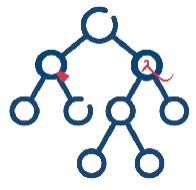
\includegraphics[height=1.0cm]{msca_logo.png}}%
    \end{center}

    \vspace{0.6cm}

    % Main title with Q logos on sides (with clickable links)
    \begin{center}
        \begin{minipage}{0.1\textwidth}
            \centering
            \href{https://quantlet.com}{
\includegraphics[height=1.1cm]{ql_logo.png}}
        \end{minipage}%
        \begin{minipage}{0.78\textwidth}
            \centering
            {\LARGE\bfseries\usebeamercolor[fg]{title}\inserttitle}

            \vspace{0.3cm}

            {\usebeamerfont{subtitle}\usebeamercolor[fg]{title}\insertsubtitle}
        \end{minipage}%
        \begin{minipage}{0.1\textwidth}
            \centering
            \href{https://quantinar.com}{
\includegraphics[height=1.1cm]{qr_logo.png}}
        \end{minipage}
    \end{center}

    \vspace{0.6cm}

    % Authors (left aligned)
    \hspace{0.5cm}{\usebeamerfont{author}\insertauthor}

    \vspace{0.3cm}

    % Institute/Affiliations (left aligned)
    \hspace{0.5cm}\begin{minipage}[t]{0.9\textwidth}
        \raggedright\small\insertinstitute
    \end{minipage}
}

%=============================================================================
% THEOREM ENVIRONMENTS
%=============================================================================
\theoremstyle{definition}
\setbeamertemplate{theorems}[numbered]
\ifdefined\sfmlang
\newtheorem{defn}{Definiție}
\newtheorem{thm}{Teoremă}
\newtheorem{prop}{Propoziție}
\newtheorem{rmk}{Observație}
\else
\newtheorem{defn}{Definition}
\newtheorem{thm}{Theorem}
\newtheorem{prop}{Proposition}
\newtheorem{rmk}{Remark}
\fi

%=============================================================================
% CENTRED MINIPAGE (no extra vertical space)
%=============================================================================
\newenvironment{cminipage}[1]{%
    \par\noindent\hfill\begin{minipage}{#1}\ignorespaces
}{%
    \end{minipage}\hfill\null\par
}

%=============================================================================
% CUSTOM COMMANDS
%=============================================================================
\newcommand{\E}{\mathbb{E}}
\newcommand{\Var}{\text{Var}}
\newcommand{\Cov}{\text{Cov}}
\newcommand{\Corr}{\text{Corr}}
\newcommand{\R}{\mathbb{R}}
\newcommand{\N}{\mathbb{N}}
\newcommand{\Z}{\mathbb{Z}}
\newcommand{\B}{\mathbf{B}}
\newcommand{\imark}{\textcolor{MainBlue}{\textbullet}}
\newcommand{\RMSE}{\text{RMSE}}
\newcommand{\MAE}{\text{MAE}}
\newcommand{\MAPE}{\text{MAPE}}

 se definește
%   \newcommand{\coursename}{Statistics of Financial Markets}      (EN)
%   \newcommand{\coursename}{Statistica piețelor financiare}       (RO)  și  \def\sfmlang{ro}
% Fișierele .tex se află în EN/Courses, EN/Seminars, RO/Cursuri, RO/Seminarii (două niveluri sub rădăcină).
% Deck-urile sînt generate de latex/build_chapterN.py / build_seminarN.py (vezi latex/sfm_build.py).

\documentclass[9pt, aspectratio=169, t]{beamer}
\providecommand{\coursename}{Statistics of Financial Markets}

% Ensure content fits on slides
\setbeamersize{text margin left=8mm, text margin right=8mm}

%=============================================================================
% THEME AND STYLE CONFIGURATION
%=============================================================================
\usetheme{default}
% Using default theme for clean header/footer control

% Color Palette (matching Redispatch PDF)
\definecolor{MainBlue}{RGB}{26, 58, 110}
\definecolor{AccentBlue}{RGB}{26, 58, 110}
\definecolor{IDAred}{RGB}{205, 0, 0}
\definecolor{DarkGray}{RGB}{51, 51, 51}
\definecolor{MediumGray}{RGB}{128, 128, 128}
\definecolor{LightGray}{RGB}{248, 248, 248}
\definecolor{VeryLightGray}{RGB}{235, 235, 235}
\definecolor{KeynoteGray}{RGB}{218, 218, 218}
\definecolor{SectionGray}{RGB}{120, 120, 120}
\definecolor{FooterGray}{RGB}{100, 100, 100}
\definecolor{Crimson}{RGB}{220, 53, 69}
\definecolor{Forest}{RGB}{46, 125, 50}
\definecolor{Amber}{RGB}{181, 133, 63}
\definecolor{Orange}{RGB}{230, 126, 34}
\definecolor{Purple}{RGB}{142, 68, 173}

% Gradient background (exact Keynote 315° gradient: white to RGB 218,218,218)
\setbeamertemplate{background}{%
    \begin{tikzpicture}[remember picture, overlay]
        \shade[shading=axis, shading angle=315,
        top color=white, bottom color=KeynoteGray]
        (current page.south west) rectangle (current page.north east);
    \end{tikzpicture}%
}
% Fallback solid color for compatibility
\setbeamercolor{background canvas}{bg=}

\setbeamercolor{palette primary}{bg=MainBlue, fg=white}
\setbeamercolor{palette secondary}{bg=MainBlue!85, fg=white}
\setbeamercolor{palette tertiary}{bg=MainBlue!70, fg=white}
\setbeamercolor{structure}{fg=MainBlue}
\setbeamercolor{title}{fg=IDAred}
\setbeamercolor{frametitle}{fg=IDAred, bg=}
\setbeamercolor{block title}{bg=MainBlue, fg=white}
\setbeamercolor{block body}{bg=VeryLightGray, fg=DarkGray}
\setbeamercolor{block title alerted}{bg=Crimson, fg=white}
\setbeamercolor{block body alerted}{bg=Crimson!8, fg=DarkGray}
\setbeamercolor{block title example}{bg=Forest, fg=white}
\setbeamercolor{block body example}{bg=Forest!8, fg=DarkGray}
\setbeamercolor{item}{fg=MainBlue}

% Footer colors (override Madrid theme blue)
\setbeamercolor{author in head/foot}{fg=FooterGray, bg=}
\setbeamercolor{title in head/foot}{fg=FooterGray, bg=}
\setbeamercolor{date in head/foot}{fg=FooterGray, bg=}
\setbeamercolor{section in head/foot}{fg=FooterGray, bg=}
\setbeamercolor{subsection in head/foot}{fg=FooterGray, bg=}

% Bullet styles (apply everywhere including blocks)
\setbeamertemplate{itemize item}{\color{MainBlue}$\boxdot$}
\setbeamertemplate{itemize subitem}{\color{MainBlue}$\blacktriangleright$}
\setbeamertemplate{itemize subsubitem}{\color{MainBlue}\tiny$\bullet$}
\setbeamertemplate{itemize/enumerate body begin}{\normalsize}
\setbeamertemplate{itemize/enumerate subbody begin}{\normalsize}

% Item spacing - compact style
\setlength{\leftmargini}{10pt}       % Level 1: minimal indent
\setlength{\leftmarginii}{10pt}      % Level 2: minimal additional indent
% Compact list spacing (zero extra space before/after lists in blocks)
\makeatletter
\def\@listi{\leftmargin\leftmargini \topsep 0pt \parsep 0pt \itemsep 0pt}
\def\@listii{\leftmargin\leftmarginii \topsep 0pt \parsep 0pt \itemsep 0pt}
\makeatother

\setbeamertemplate{navigation symbols}{}

%=============================================================================
% CUSTOM HEADLINE
%=============================================================================
\setbeamertemplate{headline}{%
    \vskip10pt%
    \hbox to \paperwidth{%
        \hskip0.5cm%
        {\small\color{FooterGray}\renewcommand{\hyperlink}[2]{##2}\insertsectionhead}%
        \hfill%
        \textcolor{FooterGray}{\small\insertframenumber}%
        \hskip0.5cm%
    }%
    \vskip4pt%
    {\color{FooterGray}\hrule height 0.4pt}%
}

%=============================================================================
% CUSTOM FOOTER
%=============================================================================
\usepackage{fontawesome5}

\setbeamertemplate{footline}{%
    {\color{FooterGray}\hrule height 0.4pt}%
    \vskip4pt%
    \hbox to \paperwidth{%
        \hskip0.5cm%
        \textcolor{FooterGray}{\small\coursename}%
        \hfill%
        \raisebox{-0.1em}{%
            \begin{tikzpicture}[x=0.08em, y=0.08em, line width=0.4pt]
                \draw[FooterGray] (0,3) -- (1,4) -- (2,3.5) -- (3,5) -- (4,4) -- (5,6) -- (6,5.5) -- (7,4) -- (8,5) -- (9,7) -- (10,6) -- (11,5) -- (12,6.5) -- (13,8) -- (14,7) -- (15,6) -- (16,7.5) -- (17,9) -- (18,8) -- (19,7) -- (20,8.5) -- (21,10) -- (22,9) -- (23,8) -- (24,9.5);
            \end{tikzpicture}%
        }%
        \hskip0.5cm%
    }%
    \vskip6pt%
}

%=============================================================================
% PACKAGES
%=============================================================================
\usepackage[utf8]{inputenc}
\DeclareUnicodeCharacter{03B1}{\ensuremath{\alpha}}
\usepackage[T1]{fontenc}
\usepackage{amsmath, amssymb, amsthm}
\usepackage{mathtools}
\usepackage{bm}
\usepackage{tikz}
\usetikzlibrary{arrows.meta, positioning, shapes, calc, decorations.pathreplacing, shadings}
\usepackage{booktabs}
\usepackage{multirow}
\usepackage{array}
\usepackage{graphicx}
\usepackage{hyperref}
\usepackage{colortbl}
\usepackage{listings}
\lstset{language=Python, basicstyle=\ttfamily\scriptsize, keywordstyle=\color{MainBlue}\bfseries,
  commentstyle=\color{Forest}, stringstyle=\color{Crimson}, breaklines=true,
  frame=none, backgroundcolor=\color{VeryLightGray}, xleftmargin=2mm}
\hypersetup{colorlinks=true, linkcolor=MainBlue, urlcolor=MainBlue}
\graphicspath{{../../logos/}{../../charts/}{../../photos/}}
\usepackage{xcolor}
\hfuzz=2pt  % Suppress tiny overfull warnings (<2pt)
\vfuzz=2pt  % Suppress tiny vertical overfull warnings (<2pt)

%=============================================================================
% QUANTLET COMMANDS
%   \quantlet{<displayed name>}{<url>}       (generic, compatible with the older SFM decks)
%   \sfmquantlet{Ch_05}{SFM_ch5_garch}       -> https://github.com/danpele/SFM/tree/main/Quantlets/Ch_05/SFM_ch5_garch
%   \qlurl{<folder>} is defined per chapter by the generator (Quantlets/Ch_NN/<folder>)
%=============================================================================
\newcommand{\sfmrepo}{https://github.com/danpele/SFM}
\newcommand{\sfmqlbase}{https://github.com/danpele/SFM/tree/main/Quantlets}
\newcommand{\quantlet}[2]{%
    \hfill\href{#2}{%
        \raisebox{-0.15em}{
\includegraphics[height=0.7em]{ql_logo.png}}%
        \textcolor{MainBlue}{\tiny\ #1}%
    }%
}
\newcommand{\sfmquantlet}[2]{\quantlet{\detokenize{#2}}{\sfmqlbase/#1/#2}}

%=============================================================================
% NOTEBOOKS (Google Colab)
%   \colaburl{notebooks/EN/chapter5_seminar_notebook.ipynb} -> the Colab link of a file in the SFM repo
%   \nb: the chapter notebook (each seminar deck redefines it with \renewcommand)
%=============================================================================
\newcommand{\colaburl}[1]{https://colab.research.google.com/github/danpele/SFM/blob/main/#1}
\newcommand{\nb}{https://colab.research.google.com/github/danpele/SFM/tree/main/notebooks/EN}
\newcommand{\nbname}{notebooks/EN}

%=============================================================================
% SLIDE HELPERS (used by the generators; the same as in MFM)
%=============================================================================
% local font size for list bodies (the preamble forces \normalsize)
\newcommand{\itemsize}[1]{\setbeamertemplate{itemize/enumerate body begin}{#1}\setbeamertemplate{itemize/enumerate subbody begin}{#1}}
\newcommand{\intitle}[1]{{\hypersetup{urlcolor=white}#1}}   % white links inside coloured title bars
\newcommand{\imgcap}[1]{{\scriptsize #1}\\[0.5mm]}          % caption under a photo
\newcommand{\imgcredit}[2]{{\tiny\color{FooterGray}\href{#1}{#2}}}   % image credit: source URL, author/licence
\newcommand{\aiprompt}[1]{{\ttfamily\color{MainBlue}#1}}     % a prompt to an AI assistant

%=============================================================================
% SEMINARS: student version by default; the instructor wrapper *_solutions.tex sets \solutionstrue
%=============================================================================
\makeatletter\@ifundefined{ifsolutions}{\expandafter\newif\csname ifsolutions\endcsname}{}\makeatother
\newcommand{\solonly}[1]{\ifsolutions #1\fi}
\newcommand{\propsub}{\ifsolutions\else\framesubtitle{\ifdefined\sfmlang Rezolvarea se discută la seminar\else Solution discussed in class\fi}\fi}

%=============================================================================
% APPENDIX AND CHAPTER LINKS (latex/appendix_links.py writes the calls; it also re-declares these
% macros before \begin{document}, so the decks compile with or without this preamble block)
%=============================================================================
\providecommand{\sfmapplink}[3]{\hypertarget{#2}{}\hyperlink{#1}{\beamergotobutton{#3}}}
\providecommand{\sfmappback}[2]{\begin{tikzpicture}[remember picture,overlay]\node[anchor=south east] at ([xshift=-3mm,yshift=7mm]current page.south east){\hyperlink{#1}{\beamerreturnbutton{#2}}};\end{tikzpicture}}
\providecommand{\sfmchlink}[2]{\href{#1}{#2}}
\providecommand{\sfmchlinkt}[2]{\href{#1}{\usebeamercolor[fg]{frametitle}#2}}

%=============================================================================
% QUANTINAR COMMAND: link către un curs Quantinar (subiecte avansate)
%=============================================================================
\newcommand{\quantinar}[2]{%
    \href{#2}{%
        \raisebox{-0.15em}{
\includegraphics[height=0.8em]{qr_logo.png}}%
        \textcolor{MainBlue}{\scriptsize\ #1}%
    }%
}

%=============================================================================
% CUSTOM TITLE PAGE
%=============================================================================
\defbeamertemplate*{title page}{hybrid}[1][]
{
    \vspace{0.2cm}
    % Logos row - top header (with clickable links)
    \begin{center}
        \href{https://www.ase.ro}{
\includegraphics[height=1.0cm]{ase_logo.png}}\hspace{0.3cm}%
        \href{https://theida.net}{
\includegraphics[height=1.0cm]{ida_logo.png}}\hspace{0.3cm}%
        \href{https://blockchain-research-center.com}{
\includegraphics[height=1.0cm]{brc_logo.png}}\hspace{0.3cm}%
        \href{https://www.ai4efin.ase.ro}{
\includegraphics[height=1.0cm]{ai4efin_logo.png}}\hspace{0.3cm}%
        \href{https://ipe.ro/new}{
\includegraphics[height=1.0cm]{acad_logo.png}}\hspace{0.3cm}%
        \href{https://www.digital-finance-msca.com}{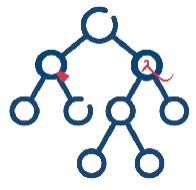
\includegraphics[height=1.0cm]{msca_logo.png}}%
    \end{center}

    \vspace{0.6cm}

    % Main title with Q logos on sides (with clickable links)
    \begin{center}
        \begin{minipage}{0.1\textwidth}
            \centering
            \href{https://quantlet.com}{
\includegraphics[height=1.1cm]{ql_logo.png}}
        \end{minipage}%
        \begin{minipage}{0.78\textwidth}
            \centering
            {\LARGE\bfseries\usebeamercolor[fg]{title}\inserttitle}

            \vspace{0.3cm}

            {\usebeamerfont{subtitle}\usebeamercolor[fg]{title}\insertsubtitle}
        \end{minipage}%
        \begin{minipage}{0.1\textwidth}
            \centering
            \href{https://quantinar.com}{
\includegraphics[height=1.1cm]{qr_logo.png}}
        \end{minipage}
    \end{center}

    \vspace{0.6cm}

    % Authors (left aligned)
    \hspace{0.5cm}{\usebeamerfont{author}\insertauthor}

    \vspace{0.3cm}

    % Institute/Affiliations (left aligned)
    \hspace{0.5cm}\begin{minipage}[t]{0.9\textwidth}
        \raggedright\small\insertinstitute
    \end{minipage}
}

%=============================================================================
% THEOREM ENVIRONMENTS
%=============================================================================
\theoremstyle{definition}
\setbeamertemplate{theorems}[numbered]
\ifdefined\sfmlang
\newtheorem{defn}{Definiție}
\newtheorem{thm}{Teoremă}
\newtheorem{prop}{Propoziție}
\newtheorem{rmk}{Observație}
\else
\newtheorem{defn}{Definition}
\newtheorem{thm}{Theorem}
\newtheorem{prop}{Proposition}
\newtheorem{rmk}{Remark}
\fi

%=============================================================================
% CENTRED MINIPAGE (no extra vertical space)
%=============================================================================
\newenvironment{cminipage}[1]{%
    \par\noindent\hfill\begin{minipage}{#1}\ignorespaces
}{%
    \end{minipage}\hfill\null\par
}

%=============================================================================
% CUSTOM COMMANDS
%=============================================================================
\newcommand{\E}{\mathbb{E}}
\newcommand{\Var}{\text{Var}}
\newcommand{\Cov}{\text{Cov}}
\newcommand{\Corr}{\text{Corr}}
\newcommand{\R}{\mathbb{R}}
\newcommand{\N}{\mathbb{N}}
\newcommand{\Z}{\mathbb{Z}}
\newcommand{\B}{\mathbf{B}}
\newcommand{\imark}{\textcolor{MainBlue}{\textbullet}}
\newcommand{\RMSE}{\text{RMSE}}
\newcommand{\MAE}{\text{MAE}}
\newcommand{\MAPE}{\text{MAPE}}

 se definește
%   \newcommand{\coursename}{Statistics of Financial Markets}      (EN)
%   \newcommand{\coursename}{Statistica piețelor financiare}       (RO)  și  \def\sfmlang{ro}
% Fișierele .tex se află în EN/Courses, EN/Seminars, RO/Cursuri, RO/Seminarii (două niveluri sub rădăcină).
% Deck-urile sînt generate de latex/build_chapterN.py / build_seminarN.py (vezi latex/sfm_build.py).

\documentclass[9pt, aspectratio=169, t]{beamer}
\providecommand{\coursename}{Statistics of Financial Markets}

% Ensure content fits on slides
\setbeamersize{text margin left=8mm, text margin right=8mm}

%=============================================================================
% THEME AND STYLE CONFIGURATION
%=============================================================================
\usetheme{default}
% Using default theme for clean header/footer control

% Color Palette (matching Redispatch PDF)
\definecolor{MainBlue}{RGB}{26, 58, 110}
\definecolor{AccentBlue}{RGB}{26, 58, 110}
\definecolor{IDAred}{RGB}{205, 0, 0}
\definecolor{DarkGray}{RGB}{51, 51, 51}
\definecolor{MediumGray}{RGB}{128, 128, 128}
\definecolor{LightGray}{RGB}{248, 248, 248}
\definecolor{VeryLightGray}{RGB}{235, 235, 235}
\definecolor{KeynoteGray}{RGB}{218, 218, 218}
\definecolor{SectionGray}{RGB}{120, 120, 120}
\definecolor{FooterGray}{RGB}{100, 100, 100}
\definecolor{Crimson}{RGB}{220, 53, 69}
\definecolor{Forest}{RGB}{46, 125, 50}
\definecolor{Amber}{RGB}{181, 133, 63}
\definecolor{Orange}{RGB}{230, 126, 34}
\definecolor{Purple}{RGB}{142, 68, 173}

% Gradient background (exact Keynote 315° gradient: white to RGB 218,218,218)
\setbeamertemplate{background}{%
    \begin{tikzpicture}[remember picture, overlay]
        \shade[shading=axis, shading angle=315,
        top color=white, bottom color=KeynoteGray]
        (current page.south west) rectangle (current page.north east);
    \end{tikzpicture}%
}
% Fallback solid color for compatibility
\setbeamercolor{background canvas}{bg=}

\setbeamercolor{palette primary}{bg=MainBlue, fg=white}
\setbeamercolor{palette secondary}{bg=MainBlue!85, fg=white}
\setbeamercolor{palette tertiary}{bg=MainBlue!70, fg=white}
\setbeamercolor{structure}{fg=MainBlue}
\setbeamercolor{title}{fg=IDAred}
\setbeamercolor{frametitle}{fg=IDAred, bg=}
\setbeamercolor{block title}{bg=MainBlue, fg=white}
\setbeamercolor{block body}{bg=VeryLightGray, fg=DarkGray}
\setbeamercolor{block title alerted}{bg=Crimson, fg=white}
\setbeamercolor{block body alerted}{bg=Crimson!8, fg=DarkGray}
\setbeamercolor{block title example}{bg=Forest, fg=white}
\setbeamercolor{block body example}{bg=Forest!8, fg=DarkGray}
\setbeamercolor{item}{fg=MainBlue}

% Footer colors (override Madrid theme blue)
\setbeamercolor{author in head/foot}{fg=FooterGray, bg=}
\setbeamercolor{title in head/foot}{fg=FooterGray, bg=}
\setbeamercolor{date in head/foot}{fg=FooterGray, bg=}
\setbeamercolor{section in head/foot}{fg=FooterGray, bg=}
\setbeamercolor{subsection in head/foot}{fg=FooterGray, bg=}

% Bullet styles (apply everywhere including blocks)
\setbeamertemplate{itemize item}{\color{MainBlue}$\boxdot$}
\setbeamertemplate{itemize subitem}{\color{MainBlue}$\blacktriangleright$}
\setbeamertemplate{itemize subsubitem}{\color{MainBlue}\tiny$\bullet$}
\setbeamertemplate{itemize/enumerate body begin}{\normalsize}
\setbeamertemplate{itemize/enumerate subbody begin}{\normalsize}

% Item spacing - compact style
\setlength{\leftmargini}{10pt}       % Level 1: minimal indent
\setlength{\leftmarginii}{10pt}      % Level 2: minimal additional indent
% Compact list spacing (zero extra space before/after lists in blocks)
\makeatletter
\def\@listi{\leftmargin\leftmargini \topsep 0pt \parsep 0pt \itemsep 0pt}
\def\@listii{\leftmargin\leftmarginii \topsep 0pt \parsep 0pt \itemsep 0pt}
\makeatother

\setbeamertemplate{navigation symbols}{}

%=============================================================================
% CUSTOM HEADLINE
%=============================================================================
\setbeamertemplate{headline}{%
    \vskip10pt%
    \hbox to \paperwidth{%
        \hskip0.5cm%
        {\small\color{FooterGray}\renewcommand{\hyperlink}[2]{##2}\insertsectionhead}%
        \hfill%
        \textcolor{FooterGray}{\small\insertframenumber}%
        \hskip0.5cm%
    }%
    \vskip4pt%
    {\color{FooterGray}\hrule height 0.4pt}%
}

%=============================================================================
% CUSTOM FOOTER
%=============================================================================
\usepackage{fontawesome5}

\setbeamertemplate{footline}{%
    {\color{FooterGray}\hrule height 0.4pt}%
    \vskip4pt%
    \hbox to \paperwidth{%
        \hskip0.5cm%
        \textcolor{FooterGray}{\small\coursename}%
        \hfill%
        \raisebox{-0.1em}{%
            \begin{tikzpicture}[x=0.08em, y=0.08em, line width=0.4pt]
                \draw[FooterGray] (0,3) -- (1,4) -- (2,3.5) -- (3,5) -- (4,4) -- (5,6) -- (6,5.5) -- (7,4) -- (8,5) -- (9,7) -- (10,6) -- (11,5) -- (12,6.5) -- (13,8) -- (14,7) -- (15,6) -- (16,7.5) -- (17,9) -- (18,8) -- (19,7) -- (20,8.5) -- (21,10) -- (22,9) -- (23,8) -- (24,9.5);
            \end{tikzpicture}%
        }%
        \hskip0.5cm%
    }%
    \vskip6pt%
}

%=============================================================================
% PACKAGES
%=============================================================================
\usepackage[utf8]{inputenc}
\DeclareUnicodeCharacter{03B1}{\ensuremath{\alpha}}
\usepackage[T1]{fontenc}
\usepackage{amsmath, amssymb, amsthm}
\usepackage{mathtools}
\usepackage{bm}
\usepackage{tikz}
\usetikzlibrary{arrows.meta, positioning, shapes, calc, decorations.pathreplacing, shadings}
\usepackage{booktabs}
\usepackage{multirow}
\usepackage{array}
\usepackage{graphicx}
\usepackage{hyperref}
\usepackage{colortbl}
\usepackage{listings}
\lstset{language=Python, basicstyle=\ttfamily\scriptsize, keywordstyle=\color{MainBlue}\bfseries,
  commentstyle=\color{Forest}, stringstyle=\color{Crimson}, breaklines=true,
  frame=none, backgroundcolor=\color{VeryLightGray}, xleftmargin=2mm}
\hypersetup{colorlinks=true, linkcolor=MainBlue, urlcolor=MainBlue}
\graphicspath{{../../logos/}{../../charts/}{../../photos/}}
\usepackage{xcolor}
\hfuzz=2pt  % Suppress tiny overfull warnings (<2pt)
\vfuzz=2pt  % Suppress tiny vertical overfull warnings (<2pt)

%=============================================================================
% QUANTLET COMMANDS
%   \quantlet{<displayed name>}{<url>}       (generic, compatible with the older SFM decks)
%   \sfmquantlet{Ch_05}{SFM_ch5_garch}       -> https://github.com/danpele/SFM/tree/main/Quantlets/Ch_05/SFM_ch5_garch
%   \qlurl{<folder>} is defined per chapter by the generator (Quantlets/Ch_NN/<folder>)
%=============================================================================
\newcommand{\sfmrepo}{https://github.com/danpele/SFM}
\newcommand{\sfmqlbase}{https://github.com/danpele/SFM/tree/main/Quantlets}
\newcommand{\quantlet}[2]{%
    \hfill\href{#2}{%
        \raisebox{-0.15em}{
\includegraphics[height=0.7em]{ql_logo.png}}%
        \textcolor{MainBlue}{\tiny\ #1}%
    }%
}
\newcommand{\sfmquantlet}[2]{\quantlet{\detokenize{#2}}{\sfmqlbase/#1/#2}}

%=============================================================================
% NOTEBOOKS (Google Colab)
%   \colaburl{notebooks/EN/chapter5_seminar_notebook.ipynb} -> the Colab link of a file in the SFM repo
%   \nb: the chapter notebook (each seminar deck redefines it with \renewcommand)
%=============================================================================
\newcommand{\colaburl}[1]{https://colab.research.google.com/github/danpele/SFM/blob/main/#1}
\newcommand{\nb}{https://colab.research.google.com/github/danpele/SFM/tree/main/notebooks/EN}
\newcommand{\nbname}{notebooks/EN}

%=============================================================================
% SLIDE HELPERS (used by the generators; the same as in MFM)
%=============================================================================
% local font size for list bodies (the preamble forces \normalsize)
\newcommand{\itemsize}[1]{\setbeamertemplate{itemize/enumerate body begin}{#1}\setbeamertemplate{itemize/enumerate subbody begin}{#1}}
\newcommand{\intitle}[1]{{\hypersetup{urlcolor=white}#1}}   % white links inside coloured title bars
\newcommand{\imgcap}[1]{{\scriptsize #1}\\[0.5mm]}          % caption under a photo
\newcommand{\imgcredit}[2]{{\tiny\color{FooterGray}\href{#1}{#2}}}   % image credit: source URL, author/licence
\newcommand{\aiprompt}[1]{{\ttfamily\color{MainBlue}#1}}     % a prompt to an AI assistant

%=============================================================================
% SEMINARS: student version by default; the instructor wrapper *_solutions.tex sets \solutionstrue
%=============================================================================
\makeatletter\@ifundefined{ifsolutions}{\expandafter\newif\csname ifsolutions\endcsname}{}\makeatother
\newcommand{\solonly}[1]{\ifsolutions #1\fi}
\newcommand{\propsub}{\ifsolutions\else\framesubtitle{\ifdefined\sfmlang Rezolvarea se discută la seminar\else Solution discussed in class\fi}\fi}

%=============================================================================
% APPENDIX AND CHAPTER LINKS (latex/appendix_links.py writes the calls; it also re-declares these
% macros before \begin{document}, so the decks compile with or without this preamble block)
%=============================================================================
\providecommand{\sfmapplink}[3]{\hypertarget{#2}{}\hyperlink{#1}{\beamergotobutton{#3}}}
\providecommand{\sfmappback}[2]{\begin{tikzpicture}[remember picture,overlay]\node[anchor=south east] at ([xshift=-3mm,yshift=7mm]current page.south east){\hyperlink{#1}{\beamerreturnbutton{#2}}};\end{tikzpicture}}
\providecommand{\sfmchlink}[2]{\href{#1}{#2}}
\providecommand{\sfmchlinkt}[2]{\href{#1}{\usebeamercolor[fg]{frametitle}#2}}

%=============================================================================
% QUANTINAR COMMAND: link către un curs Quantinar (subiecte avansate)
%=============================================================================
\newcommand{\quantinar}[2]{%
    \href{#2}{%
        \raisebox{-0.15em}{
\includegraphics[height=0.8em]{qr_logo.png}}%
        \textcolor{MainBlue}{\scriptsize\ #1}%
    }%
}

%=============================================================================
% CUSTOM TITLE PAGE
%=============================================================================
\defbeamertemplate*{title page}{hybrid}[1][]
{
    \vspace{0.2cm}
    % Logos row - top header (with clickable links)
    \begin{center}
        \href{https://www.ase.ro}{
\includegraphics[height=1.0cm]{ase_logo.png}}\hspace{0.3cm}%
        \href{https://theida.net}{
\includegraphics[height=1.0cm]{ida_logo.png}}\hspace{0.3cm}%
        \href{https://blockchain-research-center.com}{
\includegraphics[height=1.0cm]{brc_logo.png}}\hspace{0.3cm}%
        \href{https://www.ai4efin.ase.ro}{
\includegraphics[height=1.0cm]{ai4efin_logo.png}}\hspace{0.3cm}%
        \href{https://ipe.ro/new}{
\includegraphics[height=1.0cm]{acad_logo.png}}\hspace{0.3cm}%
        \href{https://www.digital-finance-msca.com}{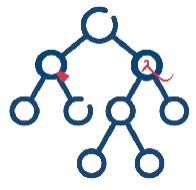
\includegraphics[height=1.0cm]{msca_logo.png}}%
    \end{center}

    \vspace{0.6cm}

    % Main title with Q logos on sides (with clickable links)
    \begin{center}
        \begin{minipage}{0.1\textwidth}
            \centering
            \href{https://quantlet.com}{
\includegraphics[height=1.1cm]{ql_logo.png}}
        \end{minipage}%
        \begin{minipage}{0.78\textwidth}
            \centering
            {\LARGE\bfseries\usebeamercolor[fg]{title}\inserttitle}

            \vspace{0.3cm}

            {\usebeamerfont{subtitle}\usebeamercolor[fg]{title}\insertsubtitle}
        \end{minipage}%
        \begin{minipage}{0.1\textwidth}
            \centering
            \href{https://quantinar.com}{
\includegraphics[height=1.1cm]{qr_logo.png}}
        \end{minipage}
    \end{center}

    \vspace{0.6cm}

    % Authors (left aligned)
    \hspace{0.5cm}{\usebeamerfont{author}\insertauthor}

    \vspace{0.3cm}

    % Institute/Affiliations (left aligned)
    \hspace{0.5cm}\begin{minipage}[t]{0.9\textwidth}
        \raggedright\small\insertinstitute
    \end{minipage}
}

%=============================================================================
% THEOREM ENVIRONMENTS
%=============================================================================
\theoremstyle{definition}
\setbeamertemplate{theorems}[numbered]
\ifdefined\sfmlang
\newtheorem{defn}{Definiție}
\newtheorem{thm}{Teoremă}
\newtheorem{prop}{Propoziție}
\newtheorem{rmk}{Observație}
\else
\newtheorem{defn}{Definition}
\newtheorem{thm}{Theorem}
\newtheorem{prop}{Proposition}
\newtheorem{rmk}{Remark}
\fi

%=============================================================================
% CENTRED MINIPAGE (no extra vertical space)
%=============================================================================
\newenvironment{cminipage}[1]{%
    \par\noindent\hfill\begin{minipage}{#1}\ignorespaces
}{%
    \end{minipage}\hfill\null\par
}

%=============================================================================
% CUSTOM COMMANDS
%=============================================================================
\newcommand{\E}{\mathbb{E}}
\newcommand{\Var}{\text{Var}}
\newcommand{\Cov}{\text{Cov}}
\newcommand{\Corr}{\text{Corr}}
\newcommand{\R}{\mathbb{R}}
\newcommand{\N}{\mathbb{N}}
\newcommand{\Z}{\mathbb{Z}}
\newcommand{\B}{\mathbf{B}}
\newcommand{\imark}{\textcolor{MainBlue}{\textbullet}}
\newcommand{\RMSE}{\text{RMSE}}
\newcommand{\MAE}{\text{MAE}}
\newcommand{\MAPE}{\text{MAPE}}



\newcommand{\qlurl}[1]{https://github.com/danpele/SFM/tree/main/Quantlets/Ch_06/#1}

% Clickable citations (DOIs verified via Crossref)

\newcommand{\refFHH}{\href{https://doi.org/10.1007/978-3-030-13751-9}{Franke, Härdle \& Hafner (2019)}}
\newcommand{\refFHHex}{\href{https://doi.org/10.1007/978-3-642-33929-5}{Borak, Härdle \& López-Cabrera (2013)}}
\newcommand{\refTsay}{\href{https://doi.org/10.1002/9780470644560}{Tsay (2010)}}
\newcommand{\refBox}{\href{https://doi.org/10.1080/01621459.1976.10480949}{Box (1976)}}
\newcommand{\refAkaike}{\href{https://doi.org/10.1109/TAC.1974.1100705}{Akaike (1974)}}
\newcommand{\refSchwarz}{\href{https://doi.org/10.1214/aos/1176344136}{Schwarz (1978)}}
\newcommand{\refKL}{\href{https://doi.org/10.1214/aoms/1177729694}{Kullback \& Leibler (1951)}}
\newcommand{\refBA}{\href{https://doi.org/10.1177/0049124104268644}{Burnham \& Anderson (2004)}}
\newcommand{\refBAbook}{\href{https://doi.org/10.1007/b97636}{Burnham \& Anderson (2002)}}
\newcommand{\refStone}{\href{https://doi.org/10.1111/j.2517-6161.1977.tb01603.x}{Stone (1977)}}
\newcommand{\refHT}{\href{https://doi.org/10.1093/biomet/76.2.297}{Hurvich \& Tsai (1989)}}
\newcommand{\refWilks}{\href{https://doi.org/10.1214/aoms/1177732360}{Wilks (1938)}}
\newcommand{\refSL}{\href{https://doi.org/10.1080/01621459.1987.10478472}{Self \& Liang (1987)}}
\newcommand{\refVuong}{\href{https://doi.org/10.2307/1912557}{Vuong (1989)}}
\newcommand{\refPearson}{\href{https://doi.org/10.1080/14786440009463897}{Pearson (1900)}}
\newcommand{\refSmirnov}{\href{https://doi.org/10.1214/aoms/1177730256}{Smirnov (1948)}}
\newcommand{\refLilliefors}{\href{https://doi.org/10.1080/01621459.1967.10482916}{Lilliefors (1967)}}
\newcommand{\refAD}{\href{https://doi.org/10.1214/aoms/1177729437}{Anderson \& Darling (1952)}}
\newcommand{\refADb}{\href{https://doi.org/10.1080/01621459.1954.10501232}{Anderson \& Darling (1954)}}
\newcommand{\refCramer}{\href{https://doi.org/10.1080/03461238.1928.10416862}{Cramér (1928)}}
\newcommand{\refStephens}{\href{https://doi.org/10.1080/01621459.1974.10480196}{Stephens (1974)}}
\newcommand{\refSGQ}{\href{https://doi.org/10.1007/BF02613687}{Stute et al.\ (1993)}}
\newcommand{\refHansen}{\href{https://doi.org/10.2307/2527081}{Hansen (1994)}}
\newcommand{\refNelson}{\href{https://doi.org/10.2307/2938260}{Nelson (1991)}}
\newcommand{\refKon}{\href{https://doi.org/10.1111/j.1540-6261.1984.tb03865.x}{Kon (1984)}}
\newcommand{\refBN}{\href{https://doi.org/10.1111/1467-9469.00045}{Barndorff-Nielsen (1997)}}
\newcommand{\refEK}{\href{https://doi.org/10.2307/3318481}{Eberlein \& Keller (1995)}}
\newcommand{\refKupiec}{\href{https://doi.org/10.3905/jod.1995.407942}{Kupiec (1995)}}
\newcommand{\refGR}{\href{https://doi.org/10.1198/016214506000001437}{Gneiting \& Raftery (2007)}}
\newcommand{\refAG}{\href{https://doi.org/10.1198/073500106000000332}{Amisano \& Giacomini (2007)}}
\newcommand{\refDPD}{\href{https://doi.org/10.1016/j.jeconom.2011.04.001}{Diks, Panchenko \& van Dijk (2011)}}
\newcommand{\refHoeting}{\href{https://doi.org/10.1214/ss/1009212519}{Hoeting et al.\ (1999)}}
\newcommand{\refDanielsson}{\href{https://doi.org/10.1016/j.jfs.2016.02.002}{Danielsson et al.\ (2016)}}
\newcommand{\refKerkhof}{\href{https://doi.org/10.1016/j.jbankfin.2009.07.025}{Kerkhof, Melenberg \& Schumacher (2010)}}
\newcommand{\refCont}{\href{https://doi.org/10.1080/713665670}{Cont (2001)}}
\newcommand{\refPeleA}{\href{https://doi.org/10.3390/e19050226}{Pele, Lazar \& Dufour (2017)}}
\newcommand{\refPeleB}{\href{https://doi.org/10.3390/e21121204}{Pele, Lazar \& Mazurencu-Marinescu-Pele (2019)}}
\newcommand{\refWang}{\href{https://doi.org/10.1038/s41586-023-06221-2}{Wang et al.\ (2023)}}

\title[Statistics of Financial Markets]{Statistics of Financial Markets}
\subtitle{Chapter 6: Model selection and risk management}
\author[D.T. Pele]{Daniel Traian PELE}
\institute{Bucharest University of Economic Studies\\
IDA Institute Digital Assets\\
Blockchain Research Center\\
AI4EFin Artificial Intelligence for Energy Finance\\
Romanian Academy, Institute for Economic Forecasting\\
MSCA Digital Finance}
\date{}

%=============================================================================
\providecommand{\sfmapplink}[3]{\hypertarget{#2}{}\hyperlink{#1}{\beamergotobutton{#3}}}  % APPLINKS-MACROS
\providecommand{\sfmappback}[2]{\begin{tikzpicture}[remember picture,overlay]\node[anchor=south east] at ([xshift=-3mm,yshift=7mm]current page.south east){\hyperlink{#1}{\beamerreturnbutton{#2}}};\end{tikzpicture}}  % APPLINKS-MACROS
\providecommand{\sfmchlink}[2]{\href{#1}{#2}}  % APPLINKS-MACROS
\providecommand{\sfmchlinkt}[2]{\href{#1}{\usebeamercolor[fg]{frametitle}#2}}  % APPLINKS-MACROS
\begin{document}
%=============================================================================

{
\setbeamertemplate{headline}{}
\setbeamertemplate{footline}{}
\begin{frame}[noframenumbering]
    \titlepage
\end{frame}
}
% BEGIN-ACRONYMS (generat de latex/acronyms.py; nu editati manual)
\begin{frame}{Acronyms used in this material}
\setbeamertemplate{itemize/enumerate body begin}{\footnotesize}
\begin{columns}[T]
\begin{column}{0.49\textwidth}
\begin{itemize}\setlength{\itemsep}{0pt}
    \item \textbf{AD}: Anderson–Darling (test)
    \item \textbf{AI}: Artificial Intelligence
    \item \textbf{AIC}: Akaike Information Criterion
    \item \textbf{BET}: Bucharest Exchange Trading (index)
    \item \textbf{BIC}: Bayesian Information Criterion
    \item \textbf{BVB}: Bursa de Valori București (the Bucharest Stock Exchange)
    \item \textbf{CDF}: Cumulative Distribution Function
    \item \textbf{COVID-19}: COronaVIrus Disease 2019
    \item \textbf{EDF}: Empirical Distribution Function
    \item \textbf{EM}: Expectation–Maximisation (algorithm)
    \item \textbf{EMA}: Exponential Moving Average
\end{itemize}
\end{column}
\begin{column}{0.49\textwidth}
\begin{itemize}\setlength{\itemsep}{0pt}
    \item \textbf{EODHD}: EOD Historical Data (market-data provider)
    \item \textbf{ES}: Expected Shortfall
    \item \textbf{FFT}: Fast Fourier Transform
    \item \textbf{GARCH}: Generalised AutoRegressive Conditional Heteroskedasticity
    \item \textbf{GED}: Generalised Error Distribution
    \item \textbf{KS}: Kolmogorov–Smirnov (test)
    \item \textbf{LR}: Likelihood Ratio
    \item \textbf{ML}: Maximum Likelihood
    \item \textbf{NIG}: Normal Inverse Gaussian (distribution)
    \item \textbf{PP}: Probability–Probability (plot)
    \item \textbf{QQ}: Quantile–Quantile (plot)
    \item \textbf{RMA}: Rectangular Moving Average
\end{itemize}
\end{column}
\end{columns}
\end{frame}
% END-ACRONYMS

\begin{frame}{Today's Question and Route}
\itemsize{\small}
\begin{itemize}
    \item \textbf{Question}: we have seven candidate distributions for daily returns; which one should a risk manager use, and how sure can we be?
    \begin{itemize}
        \item \sfmchlink{https://danpele.github.io/SFM/EN/Courses/chapter2_classical_distributions_stylised_facts.pdf}{Chapters 2}, \sfmchlink{https://danpele.github.io/SFM/EN/Courses/chapter3_alpha_stable_distributions.pdf}{3} and \sfmchlink{https://danpele.github.io/SFM/EN/Courses/chapter5_heavy_tails_evt.pdf}{5}: the Normal distribution fails; Student-t, stable laws and extreme value theory each describe part of the picture
    \end{itemize}
    \item \textbf{Route} of the chapter
    \begin{itemize}
        \item the candidates and what they must reproduce; maximum likelihood, recalled
        \item comparing models: likelihood-ratio tests, AIC and BIC
        \item checking one model: goodness-of-fit tests, PP and QQ plots
        \item the purpose decides: which model gets VaR 1\% right, in sample and out of sample
        \item overfitting and model uncertainty
    \end{itemize}
\end{itemize}
\end{frame}

\begin{frame}{Learning Outcomes}
\itemsize{\small}
\begin{itemize}
    \item Write the log-likelihood of a candidate model and explain how maximum likelihood estimates are found
    \item Test a restricted model against a larger one with the likelihood-ratio test, and know when the test does not apply
    \item Compute AIC, BIC, $\Delta$AIC and Akaike weights and interpret them
    \item Run and read KS, Cramér--von Mises and Anderson--Darling tests, PP and QQ plots, and explain why KS is weak in the tails
    \item Judge a model by its VaR 1\% out of sample, recognise overfitting, and report model uncertainty
\end{itemize}
\end{frame}

\begin{frame}{Reading and Tools}
\itemsize{\small}
\begin{itemize}
    \item Textbook: \refFHH, Ch.~16 (Value at Risk and backtesting) and Ch.~18 (statistics of extreme risks); exercises: \refFHHex
    \begin{itemize}
        \item distributional properties of returns: \refTsay, Ch.~1
    \end{itemize}
    \item Model selection: \refBAbook; short version \refBA
    \item Goodness of fit: \refStephens; the original papers \refAD, \refLilliefors
    \item Python Quantlets of this chapter: \href{https://github.com/danpele/SFM/tree/main/Quantlets/Ch_06}{Quantlets/Ch\_06}
    \begin{itemize}
        \item ported from the Quantlets SFESumm and SFEVaRqqplot; each chart links to the Quantlet that draws it
    \end{itemize}
    \item Lecture notebook: \href{\colaburl{notebooks/EN/chapter6_lecture_notebook.ipynb}}{open in Google Colab}
    \item Video course: \quantinar{Measuring Statistical Risk}{https://quantinar.com/course/100080/measuring-statistical-risk}
\end{itemize}
\end{frame}


%=============================================================================
\section{The Candidates}
%=============================================================================

\begin{frame}{``All Models Are Wrong''}
\itemsize{\small}
\begin{columns}[T]
\begin{column}{0.62\textwidth}
\begin{itemize}
    \item George Box: a statistician should look for a model that is useful, not one that is true \refBox
    \begin{itemize}
        \item ``all models are wrong, but some are useful'' is the short form of his argument
    \end{itemize}
    \item For returns, ``useful'' depends on the purpose
    \begin{itemize}
        \item pricing and portfolio choice: the body of the distribution (typical days)
        \item risk management: the left tail (the worst 1\% of days)
    \end{itemize}
    \item This chapter: a toolbox to compare models, and the habit of asking ``useful for what?''
\end{itemize}
\end{column}
\begin{column}{0.34\textwidth}
\centering
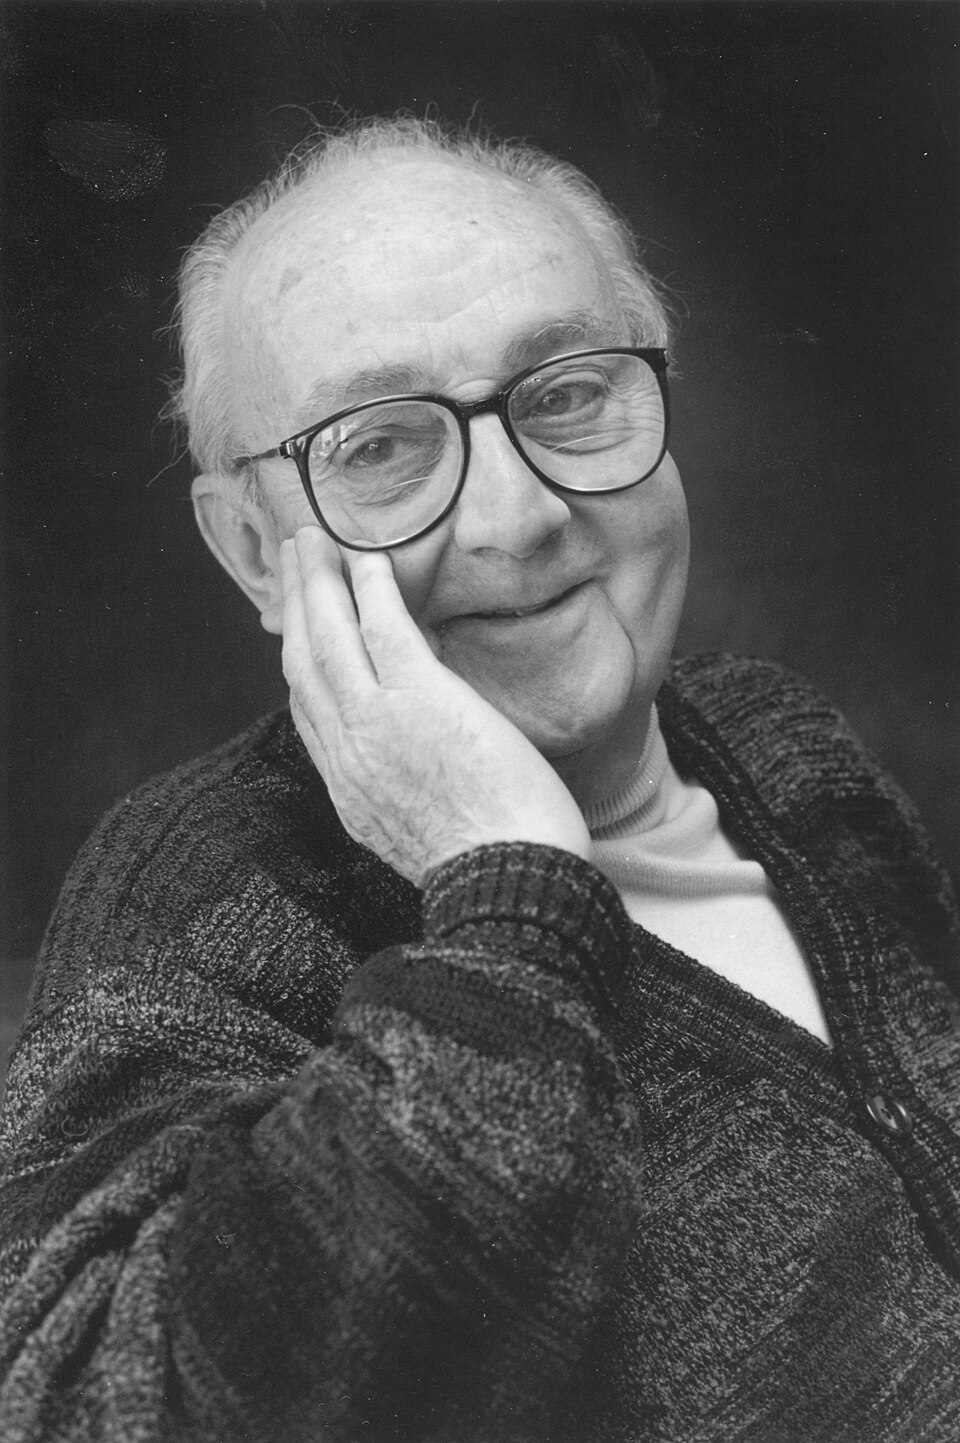
\includegraphics[height=0.46\textheight]{ch6_box.jpg}\\[1mm]
\imgcap{George E. P. Box (1919--2013)}
\imgcredit{https://commons.wikimedia.org/wiki/File:GeorgeEPBox.jpg}{Photo: DavidMCEddy (2011); CC BY-SA 3.0; Wikimedia Commons}
\end{column}
\end{columns}
\end{frame}

\begin{frame}{Seven Candidate Distributions}
\itemsize{\footnotesize}
\begin{center}
\scriptsize
\begin{tabular}{l>{\raggedright\arraybackslash}p{0.8cm}>{\raggedright\arraybackslash}p{3.2cm}>{\raggedright\arraybackslash}p{2.4cm}>{\raggedright\arraybackslash}p{2.6cm}}
\toprule
\textbf{Model} & \textbf{$k$} & \textbf{Tails} & \textbf{Skewness} & \textbf{Reference} \\
\midrule
Normal & 2 & thin, $e^{-x^2/2}$ & no & \sfmchlink{https://danpele.github.io/SFM/EN/Courses/chapter2_classical_distributions_stylised_facts.pdf}{Chapter 2} \\
Student-t & 3 & power, $x^{-\nu}$ & no & \sfmchlink{https://danpele.github.io/SFM/EN/Courses/chapter2_classical_distributions_stylised_facts.pdf}{Chapter 2} \\
skewed-t & 4 & power, $x^{-\nu}$ & yes ($\lambda$) & \refHansen{} \\
GED & 3 & $e^{-|x|^\beta}$, heavy if $\beta < 2$ & no & \refNelson{} \\
Normal mixture & 5 & thin, but a wide component & yes & \refKon{} \\
NIG & 4 & semi-heavy, $|x|^{-3/2}e^{-c|x|}$ & yes & \refBN{} \\
stable & 4 & power, $x^{-\alpha}$, $\alpha < 2$ & yes ($\beta$) & \sfmchlink{https://danpele.github.io/SFM/EN/Courses/chapter3_alpha_stable_distributions.pdf}{Chapter 3} \\
\bottomrule
\end{tabular}
\end{center}
\begin{itemize}
    \item $k$: number of parameters; GED: generalised error distribution; NIG: normal inverse Gaussian, a member of the generalised hyperbolic family \refEK
    \item Normal mixture: with probability $w$ a calm-day $N(\mu_1, \sigma_1^2)$, otherwise a turbulent-day $N(\mu_2, \sigma_2^2)$
\end{itemize}
\end{frame}

\begin{frame}{The Candidates Side by Side}
\itemsize{\footnotesize}
\begin{center}
    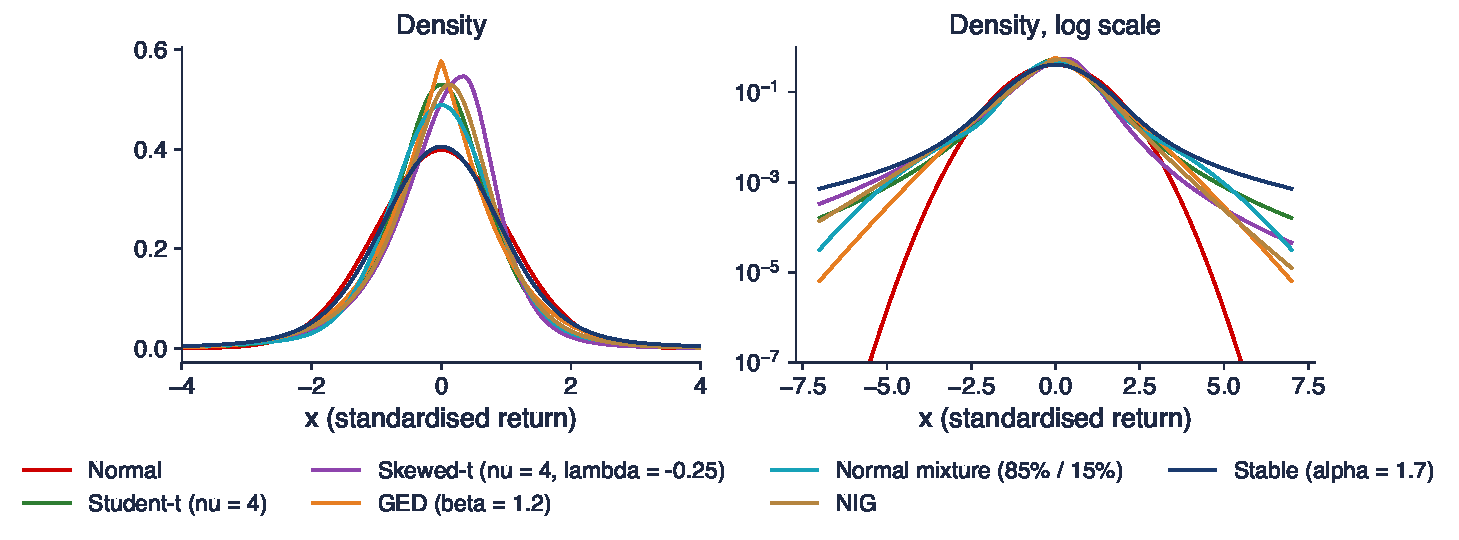
\includegraphics[width=0.97\textwidth,height=0.58\textheight,keepaspectratio]{sfm_ch6_candidates.pdf}
\end{center}
\vspace{-0.25cm}
\begin{itemize}
    \item All with mean 0 and variance 1 (stable: the same interquartile range as the Normal law); right panel on a log scale
    \item Near the centre they look alike; in the tails they differ by orders of magnitude
\end{itemize}
\quantlet{SFM\_ch6\_candidates}{\qlurl{SFM_ch6_candidates}}
\end{frame}

\begin{frame}{Same Variance, Very Different Tails}
\itemsize{\small}
\begin{itemize}
    \item $P(X < -4)$, a move of four standard deviations, under each candidate of the chart:
    \begin{itemize}
        \item Normal $3.2 \times 10^{-5}$; GED $9.5 \times 10^{-4}$; Student-t $2.4 \times 10^{-3}$; Normal mixture $2.5 \times 10^{-3}$
        \item NIG $3.2 \times 10^{-3}$; skewed-t $4.5 \times 10^{-3}$; stable $8.1 \times 10^{-3}$
    \end{itemize}
    \item The Student-t gives this loss about $76$ times the Normal probability
    \item A risk measure such as VaR 1\% lives exactly where the candidates disagree
    \item \textbf{Question for the room}: if all fit the centre well, why not keep the simplest one?
    \item \textbf{Answer}
    \begin{itemize}
        \item the simplest one (Normal) is wrong precisely in the region that drives capital and margin requirements
    \end{itemize}
\end{itemize}
\end{frame}

\begin{frame}{What Every Model Must Reproduce: the SFESumm Statistics}
\itemsize{\footnotesize}
\begin{center}
    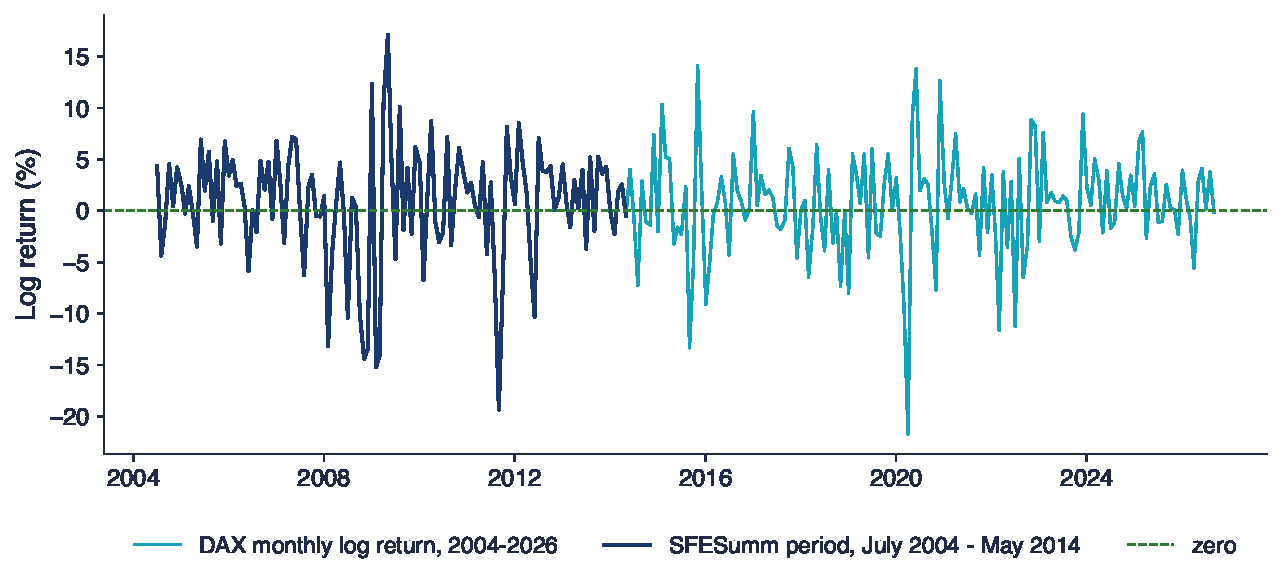
\includegraphics[width=0.97\textwidth,height=0.56\textheight,keepaspectratio]{sfm_ch6_dax_monthly.pdf}
\end{center}
\vspace{-0.25cm}
\begin{itemize}
    \item Quantlet SFESumm: DAX monthly log returns between first trading days, July 2004 -- May 2014 ($n = 119$), extended here to 1 Sep 2026
    \item Even monthly returns are skewed and heavy-tailed: the next slide gives the numbers
\end{itemize}
\quantlet{SFM\_ch6\_summary}{\qlurl{SFM_ch6_summary}}
\end{frame}

\begin{frame}{Summary Statistics: Monthly DAX and Daily Returns}
\itemsize{\footnotesize}
\begin{center}
\footnotesize
\begin{tabular}{lrrrrrrr}
\toprule
& $n$ & min & max & st.\ dev. & ann.\ vol. & skew. & kurt. \\
\midrule
DAX 2004--2014 & 119 & $-19.35$ & $17.12$ & $5.80$ & $20.08$ & $-0.83$ & $4.60$ \\
DAX 2004--2026 & 267 & $-21.70$ & $17.12$ & $5.39$ & $18.66$ & $-0.72$ & $5.06$ \\
\bottomrule
\end{tabular}
\end{center}
\begin{itemize}
    \item Monthly, in \%; st.\ dev.: standard deviation $\sigma$; ann.\ vol.: $\sigma\sqrt{12}$
    \begin{itemize}
        \item skewness $E(X - \mu)^3/\sigma^3$ and kurtosis $E(X - \mu)^4/\sigma^4$, with $\mu$ the mean; 0 and 3 for the Normal distribution
        \item Jarque--Bera test of Normality (\sfmchlink{https://danpele.github.io/SFM/EN/Courses/chapter2_classical_distributions_stylised_facts.pdf}{Chapter 2}): $p$-value $<0.001$
    \end{itemize}
    \item Daily log returns since 2000 (Bitcoin since 2014, BVB stocks since 2010): kurtosis
    \begin{itemize}
        \item BET $14.1$, S\&P 500 $13.7$, DAX $9.1$, Bitcoin $15.0$, TLV $16.5$, SNP $11.9$, BRD $10.3$
        \item skewness: S\&P 500 $-0.35$, BET $-0.65$, Bitcoin $-0.70$
    \end{itemize}
\end{itemize}\quantlet{SFM\_ch6\_summary}{\qlurl{SFM_ch6_summary}}
\end{frame}

\begin{frame}{Data Before Models: Two Bad Days}
\itemsize{\small}
\begin{itemize}
    \item Banca Transilvania (TLV), adjusted close from EODHD: log returns of $-15.0\%$ on 30 May 2016 and $20.5\%$ on 31 May 2016
    \begin{itemize}
        \item the adjustment for the bonus shares is applied one day late (\sfmchlink{https://danpele.github.io/SFM/EN/Courses/chapter2_classical_distributions_stylised_facts.pdf}{Chapter 2}): a fake crash followed by a fake rally
    \end{itemize}
    \item Effect of the two days on the fitted model
    \begin{itemize}
        \item kurtosis $20.5$ with them, $16.5$ without; Student-t $\hat\nu$: $3.33$ vs $3.44$
        \item the AIC ranking does not change here (best: Student-t), but the moments do
    \end{itemize}
    \item Rule: check the largest returns against the close and the news before any model selection; the two days are removed in the rest of the chapter
\end{itemize}
\end{frame}

\begin{frame}{Recap: The Candidates}
\itemsize{\small}
\begin{itemize}
    \item Seven candidates with 2 to 5 parameters; they agree in the centre and disagree in the tails
    \item Any model must reproduce skewness and kurtosis well above 3, even for monthly returns
    \item Clean the data first: two wrong prices raised the TLV kurtosis by about $19\%$ of its value
\end{itemize}
\end{frame}


%=============================================================================
\section{Maximum Likelihood, Recalled}
%=============================================================================

\begin{frame}{Likelihood and Log-Likelihood}
\itemsize{\footnotesize}
\begin{itemize}
    \item Data $r_1, \dots, r_n$, assumed i.i.d.\ (independent, identically distributed) with density $f(r; \theta)$
    \begin{itemize}
        \item $\theta$: the vector of model parameters (for example $\mu, \sigma$); $f$: the density of the model
        \item \textbf{likelihood}: $L(\theta) = \prod_{t=1}^n f(r_t; \theta)$, the probability density of the observed sample as a function of $\theta$
        \item \textbf{log-likelihood}: $\ell(\theta) = \sum_{t=1}^n \ln f(r_t; \theta)$; sums are easier than products
    \end{itemize}
    \item \textbf{Maximum likelihood (ML) estimate}: $\hat\theta = \arg\max_\theta \ell(\theta)$
    \begin{itemize}
        \item $\ell(\hat\theta)$, the maximised log-likelihood, is the raw material of every comparison in this chapter
    \end{itemize}
    \item Large $n$: $\hat\theta$ is approximately Normal around the true $\theta$
    \begin{itemize}
        \item covariance $\approx [-\partial^2\ell/\partial\theta\,\partial\theta^\top]^{-1}$, the inverse of the observed information
        \item a sharply curved $\ell$ (large second derivative) means a precise estimate
    \end{itemize}
\end{itemize}
\end{frame}

\begin{frame}{Worked Example: the Normal Model, Step by Step}
\itemsize{\small}
\begin{itemize}
    \item $\ell(\mu, \sigma) = -\dfrac{n}{2}\ln(2\pi\sigma^2) - \dfrac{1}{2\sigma^2}\sum_t (r_t - \mu)^2$
    \begin{itemize}
        \item setting the derivatives to zero: $\hat\mu = \bar r$, $\hat\sigma^2 = \frac{1}{n}\sum_t (r_t - \bar r)^2$ (divisor $n$, not $n - 1$)
        \item plugging back: $\ell(\hat\theta) = -\dfrac{n}{2}\big[\ln(2\pi\hat\sigma^2) + 1\big]$
    \end{itemize}
    \item S\&P 500, daily log returns in \%, 2000--2026: $n = 6\,714$, $\hat\mu = 0.025$, $\hat\sigma = 1.213$
    \begin{itemize}
        \item $\ln(2\pi\hat\sigma^2) = 2.2240$, so $\ell(\hat\theta) = -\frac{6\,714}{2}(2.2240 + 1) = -10\,823$
    \end{itemize}
    \item Only the Normal model has a closed form; the others are maximised numerically
\end{itemize}
\end{frame}

\begin{frame}{Numerical ML for the Other Candidates (S\&P 500)}
\itemsize{\footnotesize}
\begin{center}
\scriptsize
\begin{tabular}{l>{\raggedright\arraybackslash}p{6.6cm}r}
\toprule
\textbf{Model} & \textbf{Estimates} & $\ell(\hat\theta)$ \\
\midrule
Normal & $\hat\mu = 0.025$, $\hat\sigma = 1.213$ & $-10\,823$ \\
Student-t & $\hat\nu = 2.67$, location $0.068$, scale $0.703$ & $-9\,848$ \\
skewed-t & $\hat\nu = 2.69$, $\hat\lambda = -0.067$, $\hat\mu = 0.024$, $\hat\sigma = 1.39$ & $-9\,838$ \\
GED & $\hat\beta = 0.88$, location $0.068$, scale $0.653$ & $-9\,854$ \\
Normal mixture & $\hat w = 79\%$: $N(0.089, 0.71^2)$; $21\%$: $N(-0.223, 2.26^2)$ & $-9\,925$ \\
NIG & $\hat a = 0.403$, $\hat b = -0.048$, location $0.115$, scale $0.755$ & $-9\,824$ \\
stable & $\hat\alpha = 1.540$, $\hat\beta = -0.181$, $\hat\gamma = 0.582$, $\hat\delta_0 = 0.093$ & $-9\,893$ \\
\bottomrule
\end{tabular}
\end{center}
\begin{itemize}
    \item Optimiser: Nelder--Mead on transformed parameters (for example $\ln\sigma$, $\ln(\nu - 2)$); the Normal mixture by the EM (expectation--maximisation) algorithm; the stable density by FFT (\sfmchlink{https://danpele.github.io/SFM/EN/Courses/chapter3_alpha_stable_distributions.pdf}{Chapter 3})
    \item Skewed-t: $\mu$ and $\sigma$ are the mean and the standard deviation (Hansen's parameterisation)
\end{itemize}\quantlet{SFM\_ch6\_ml\_fits}{\qlurl{SFM_ch6_ml_fits}}
\end{frame}

\begin{frame}{Reading the Estimates}
\itemsize{\small}
\begin{itemize}
    \item Student-t $\hat\nu = 2.67$: tails like $x^{-2.67}$; the variance exists ($\nu > 2$), the kurtosis does not ($\nu < 4$)
    \begin{itemize}
        \item the sample kurtosis $13.7$ estimates a quantity that the fitted model says is infinite
    \end{itemize}
    \item Skewed-t $\hat\lambda = -0.067 < 0$: a slightly longer left tail (crashes)
    \item GED $\hat\beta = 0.88$: below 2 (Normal) and even below 1 (Laplace): a sharp peak
    \item Normal mixture: $79\%$ calm days with standard deviation $0.71\%$, $21\%$ turbulent days with $2.26\%$ and a negative mean
    \item Stable $\hat\alpha = 1.540$ (\sfmchlink{https://danpele.github.io/SFM/EN/Courses/chapter3_alpha_stable_distributions.pdf}{Chapter 3}): heavier tails than any other candidate
\end{itemize}
\end{frame}

\begin{frame}{How Precise Is $\hat\nu$? The Profile Log-Likelihood}
\itemsize{\footnotesize}
\begin{center}
    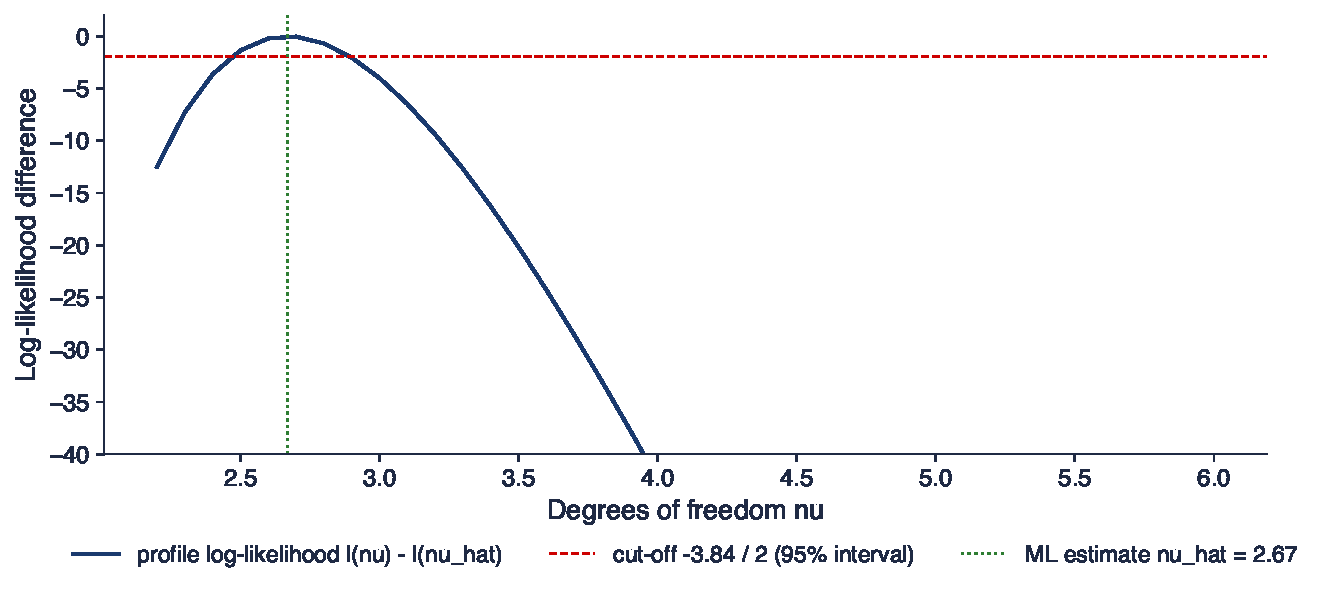
\includegraphics[width=0.97\textwidth,height=0.56\textheight,keepaspectratio]{sfm_ch6_profile_nu.pdf}
\end{center}
\vspace{-0.25cm}
\begin{itemize}
    \item For each $\nu$, maximise $\ell$ over location and scale; the curve falls by $-92$ at $\nu = 5$
    \item 95\% interval: all $\nu$ with $2[\ell(\hat\nu) - \ell(\nu)] \le 3.84$, here $[2.5, 2.8]$ around $\hat\nu = 2.67$: the tails are pinned down well
\end{itemize}
\quantlet{SFM\_ch6\_ml\_fits}{\qlurl{SFM_ch6_ml_fits}}
\end{frame}

\begin{frame}{Pitfalls of Numerical ML}
\itemsize{\small}
\begin{itemize}
    \item \textbf{Local maxima}: the optimiser can stop on a hill that is not the highest
    \begin{itemize}
        \item remedy: several starting values (the mixtures in this chapter use 4 to 12 starts)
    \end{itemize}
    \item \textbf{Boundaries}: $\nu \to 2$, a mixture weight $\to 0$, $|\lambda| \to 1$
    \begin{itemize}
        \item the usual standard errors and tests are not valid at a boundary (next section)
    \end{itemize}
    \item \textbf{Parameterisation}: the same law, different parameters
    \begin{itemize}
        \item scipy's Student-t scale is not the standard deviation: $\mathrm{sd} = \mathrm{scale}\sqrt{\nu/(\nu - 2)}$
    \end{itemize}
    \item \textbf{Check}: compare $\ell(\hat\theta)$ of nested models; a larger model can never have a lower maximum
\end{itemize}
\end{frame}

\begin{frame}{Recap: Maximum Likelihood}
\itemsize{\small}
\begin{itemize}
    \item $\ell(\theta) = \sum_t \ln f(r_t; \theta)$; the ML estimate maximises it
    \item Normal: closed form, $\ell(\hat\theta) = -\frac{n}{2}[\ln(2\pi\hat\sigma^2) + 1]$; the others: numerical
    \item Precision from the curvature of $\ell$ or from the profile log-likelihood
    \item Watch local maxima, boundaries and parameterisations
\end{itemize}
\end{frame}


%=============================================================================
\section{Nested Models: the Likelihood-Ratio Test}
%=============================================================================

\begin{frame}{Nested Models}
\itemsize{\small}
\begin{itemize}
    \item Model 0 is \textbf{nested} in model 1 if model 0 is model 1 with some parameters fixed
    \begin{itemize}
        \item Normal inside GED: $\beta = 2$
        \item Student-t inside skewed-t: $\lambda = 0$
        \item Normal inside Student-t: $\nu = \infty$, i.e.\ $1/\nu = 0$, on the \textbf{edge} of the parameter space
    \end{itemize}
    \item Not nested: Student-t and GED, Student-t and stable, skewed-t and NIG
    \begin{itemize}
        \item neither is a special case of the other: they need other tools (Vuong test, AIC)
    \end{itemize}
    \item Nested: $\ell_1(\hat\theta_1) \ge \ell_0(\hat\theta_0)$ always; the question is whether the gain is larger than chance
\end{itemize}
\end{frame}

\begin{frame}{The Likelihood-Ratio Test}
\itemsize{\small}
\begin{itemize}
    \item $H_0$: model 0 (restricted) is true; $H_1$: model 1 (larger)
    \begin{itemize}
        \item $LR = 2\,[\ell_1(\hat\theta_1) - \ell_0(\hat\theta_0)] \ge 0$: twice the gain in maximised log-likelihood
        \item $\ell_0, \ell_1$: the log-likelihoods of the two models; $k_0, k_1$: their numbers of parameters
    \end{itemize}
    \item \textbf{Wilks' theorem} (\refWilks): under $H_0$, $LR \approx \chi^2(d)$, with $d = k_1 - k_0$ restrictions
    \begin{itemize}
        \item $\chi^2(d)$: the chi-square distribution with $d$ degrees of freedom
        \item valid if the restricted values are inside the parameter space
    \end{itemize}
    \item Decision at 5\%: reject $H_0$ if $LR > \chi^2_{0.95}(d)$
    \begin{itemize}
        \item $\chi^2_{0.95}(1) = 3.84$, $\chi^2_{0.95}(2) = 5.99$
    \end{itemize}
    \item Intuition: twice the log of how many times more likely the data are under the larger model
\end{itemize}
\end{frame}

\begin{frame}{Worked Example: Is the Skewness Parameter Needed?}
\itemsize{\small}
\begin{itemize}
    \item S\&P 500: $\ell$(Student-t) $= -9\,848$, $\ell$(skewed-t) $= -9\,838$
    \begin{itemize}
        \item $LR = 2(-9\,838 - (-9\,848)) = 19.63 > 3.84$; $p <0.001$: reject $\lambda = 0$
    \end{itemize}
    \item The same test elsewhere
    \begin{itemize}
        \item DAX: $LR = 20.92$, $p <0.001$: skewness needed
        \item BET: $LR = 0.35$, $p = 0.555$; Bitcoin: $LR = 0.42$, $p = 0.515$: no evidence of skewness
    \end{itemize}
    \item Normal inside GED ($\beta = 2$): $LR$ between 1\,431 (Bitcoin) and 2\,298 (BET); the Normal model is rejected everywhere
    \item Interpretation: the two developed indices have a longer left tail; the BET and Bitcoin do not
\end{itemize}\quantlet{SFM\_ch6\_lr\_aic}{\qlurl{SFM_ch6_lr_aic}}
\end{frame}

\begin{frame}{A Boundary Case: Normal inside Student-t}
\itemsize{\small}
\begin{itemize}
    \item $H_0$: $1/\nu = 0$ is on the edge of the space $1/\nu \ge 0$: Wilks' theorem does not apply
    \begin{itemize}
        \item \refSL: the null law is a 50:50 mixture of $\chi^2(0)$ (a point mass at 0) and $\chi^2(1)$
        \item 5\% critical value: $\chi^2_{0.90}(1) = 2.71$ instead of $3.84$; the naive $p$-value is twice the correct one
    \end{itemize}
    \item Real data: $LR$ = 1\,949 (S\&P 500), 1\,337 (Bitcoin): the Normal model is rejected with either critical value
    \item The same issue appears for a mixture weight $w = 0$ and for variance parameters equal to 0
    \item \textbf{What do you think?} Does the boundary matter when $LR$ is in the thousands?
    \item \textbf{Answer}
    \begin{itemize}
        \item no for the decision; yes for small samples and borderline $LR$ values, where it halves the $p$-value
    \end{itemize}
\end{itemize}
\end{frame}

\begin{frame}{Non-Nested Models: the Vuong Test}
\itemsize{\footnotesize}
\begin{center}
\footnotesize
\begin{tabular}{lrrr}
\toprule
& Student-t vs GED & Student-t vs stable & skewed-t vs NIG \\
\midrule
BET & $3.70$ ($<0.001$) & $9.33$ ($<0.001$) & $-1.34$ ($0.179$) \\
S\&P 500 & $0.40$ ($0.686$) & $6.52$ ($<0.001$) & $-2.20$ ($0.028$) \\
DAX & $-0.23$ ($0.817$) & $7.66$ ($<0.001$) & $-2.97$ ($0.003$) \\
Bitcoin & $-3.80$ ($<0.001$) & $16.47$ ($<0.001$) & $-6.76$ ($<0.001$) \\
\bottomrule
\end{tabular}
\end{center}
\begin{itemize}
    \item \refVuong: $m_t = \ln f_1(r_t) - \ln f_2(r_t)$, $V = \sqrt{n}\,\bar m / s_m \approx N(0, 1)$ if both models are equally close to the truth
    \begin{itemize}
        \item $f_1, f_2$: the two fitted densities; $m_t$: by how much model 1 explains day $t$ better; $\bar m$, $s_m$: mean and standard deviation of the $m_t$
        \item $V > 1.96$: the first model is closer; $V < -1.96$: the second; ($p$-value) in brackets
    \end{itemize}
    \item Student-t beats the stable law everywhere; NIG beats the skewed-t on the S\&P 500 and the DAX; Student-t vs GED splits by market
\end{itemize}\quantlet{SFM\_ch6\_lr\_aic}{\qlurl{SFM_ch6_lr_aic}}
\end{frame}

\begin{frame}{Recap: Likelihood-Ratio and Vuong Tests}
\itemsize{\small}
\begin{itemize}
    \item Nested models: $LR = 2(\ell_1 - \ell_0) \approx \chi^2(k_1 - k_0)$ (Wilks)
    \item On a boundary (Normal inside Student-t): 50:50 mixture, critical value $2.71$
    \item Non-nested models: Vuong test on the pointwise log-likelihood differences
    \item Skewness matters for the S\&P 500 and DAX, not for the BET and Bitcoin
\end{itemize}
\end{frame}


%=============================================================================
\section{Information Criteria: AIC and BIC}
%=============================================================================

\begin{frame}{Akaike's Idea}
\itemsize{\small}
\begin{columns}[T]
\begin{column}{0.64\textwidth}
\begin{itemize}
    \item Hirotugu Akaike asked: which model will predict \textbf{new} data best?
    \begin{itemize}
        \item the distance from the truth $g$ to a model $f$: the Kullback--Leibler divergence \refKL
        \item $KL(g, f) = E_g[\ln g(R) - \ln f(R)] \ge 0$, zero only if $f = g$
        \item $R$: a new return drawn from the truth $g$; $E_g$: the mean under $g$
    \end{itemize}
    \item $\ell(\hat\theta)$ is too optimistic: the same data choose $\hat\theta$ and judge it
    \begin{itemize}
        \item the optimism is about $k$, the number of parameters \refAkaike
    \end{itemize}
    \item Result: $\mathrm{AIC} = -2\ell(\hat\theta) + 2k$, an estimate of the expected out-of-sample fit (lower is better)
\end{itemize}
\end{column}
\begin{column}{0.32\textwidth}
\centering
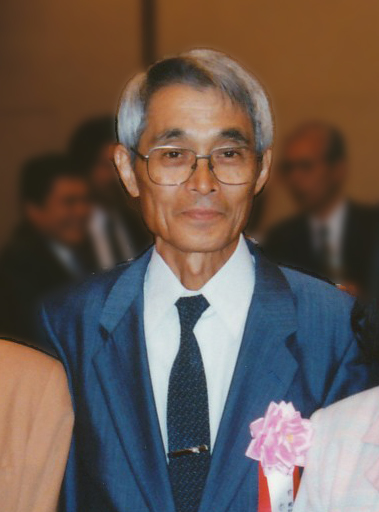
\includegraphics[height=0.44\textheight]{ch6_akaike.jpg}\\[1mm]
\imgcap{Hirotugu Akaike (1927--2009)}
\imgcredit{https://commons.wikimedia.org/wiki/File:Akaike.jpg}{Photo: The Institute of Statistical Mathematics; CC BY-SA 4.0; Wikimedia Commons}
\end{column}
\end{columns}
\end{frame}

\begin{frame}{AIC and BIC}
\itemsize{\small}
\begin{itemize}
    \item \textbf{AIC} (Akaike information criterion): $\mathrm{AIC} = -2\ell(\hat\theta) + 2k$
    \begin{itemize}
        \item aim: the best predictive model; asymptotically equivalent to leave-one-out cross-validation \refStone
        \item small samples: AICc $= \mathrm{AIC} + 2k(k+1)/(n - k - 1)$ \refHT
    \end{itemize}
    \item \textbf{BIC} (Bayesian information criterion) \refSchwarz: $\mathrm{BIC} = -2\ell(\hat\theta) + k\ln n$
    \begin{itemize}
        \item aim: the true model, if it is among the candidates (consistency)
        \item penalty per parameter $\ln n$: $8.81$ for $n = 6\,714$, more than four times the AIC penalty 2
    \end{itemize}
    \item Both: lower is better; only differences between models on the \textbf{same data} mean anything
\end{itemize}
\end{frame}

\begin{frame}{$\Delta$AIC and Akaike Weights}
\itemsize{\small}
\begin{itemize}
    \item $\Delta_i = \mathrm{AIC}_i - \min_j \mathrm{AIC}_j$; rules of thumb of \refBA:
    \begin{itemize}
        \item $\Delta \le 2$: substantial support; $4 \le \Delta \le 7$: considerably less; $\Delta > 10$: essentially none
    \end{itemize}
    \item \textbf{Akaike weight}: $w_i = \dfrac{e^{-\Delta_i/2}}{\sum_j e^{-\Delta_j/2}}$
    \begin{itemize}
        \item the weight of evidence for model $i$ among the candidates; the weights sum to 1
        \item two models with $\Delta = 0$ and $\Delta = 2$: $w = 1/(1 + e^{-1}) \approx 0.73$ and $0.27$
    \end{itemize}
    \item \textbf{What do you think?} Is $\Delta = 2$ a ``significant'' difference?
    \item \textbf{Answer}
    \begin{itemize}
        \item no: AIC is not a test; a gap of 2 means both models remain plausible (roughly 73\% vs 27\%)
    \end{itemize}
\end{itemize}
\end{frame}

\begin{frame}{Worked Example: Seven Models for the S\&P 500}
\itemsize{\footnotesize}
\begin{center}
\scriptsize
\begin{tabular}{lrrrrrrr}
\toprule
& $k$ & $\ell(\hat\theta)$ & AIC & BIC & $\Delta$AIC & $\Delta$BIC & $w$ \\
\midrule
Normal & 2 & $-10\,823$ & $21\,650$ & $21\,663$ & $1993.2$ & $1979.6$ & $0.000$ \\
Student-t & 3 & $-9\,848$ & $19\,702$ & $19\,723$ & $45.7$ & $38.9$ & $0.000$ \\
skewed-t & 4 & $-9\,838$ & $19\,685$ & $19\,712$ & $28.1$ & $28.1$ & $0.000$ \\
GED & 3 & $-9\,854$ & $19\,714$ & $19\,735$ & $57.9$ & $51.1$ & $0.000$ \\
Normal mixture & 5 & $-9\,925$ & $19\,859$ & $19\,893$ & $202.5$ & $209.3$ & $0.000$ \\
NIG & 4 & $-9\,824$ & $19\,657$ & $19\,684$ & $0.0$ & $0.0$ & $1.000$ \\
stable & 4 & $-9\,893$ & $19\,794$ & $19\,821$ & $137.3$ & $137.3$ & $0.000$ \\
\bottomrule
\end{tabular}
\end{center}
\begin{itemize}
    \item Example: NIG, $\mathrm{AIC} = -2(-9\,824) + 2 \cdot 4 = 19\,657$
    \item NIG wins on both criteria; the next model, skewed-t, has $\Delta = 28.1$, so $e^{-\Delta/2} \approx 8.1 \times 10^{-7}$: weight $w \approx 1$ for NIG
    \item Normal: $\Delta$AIC of 1\,993; the stable law: 137
\end{itemize}\quantlet{SFM\_ch6\_lr\_aic}{\qlurl{SFM_ch6_lr_aic}}
\end{frame}

\begin{frame}{$\Delta$AIC across Seven Series}
\itemsize{\footnotesize}
\begin{center}
    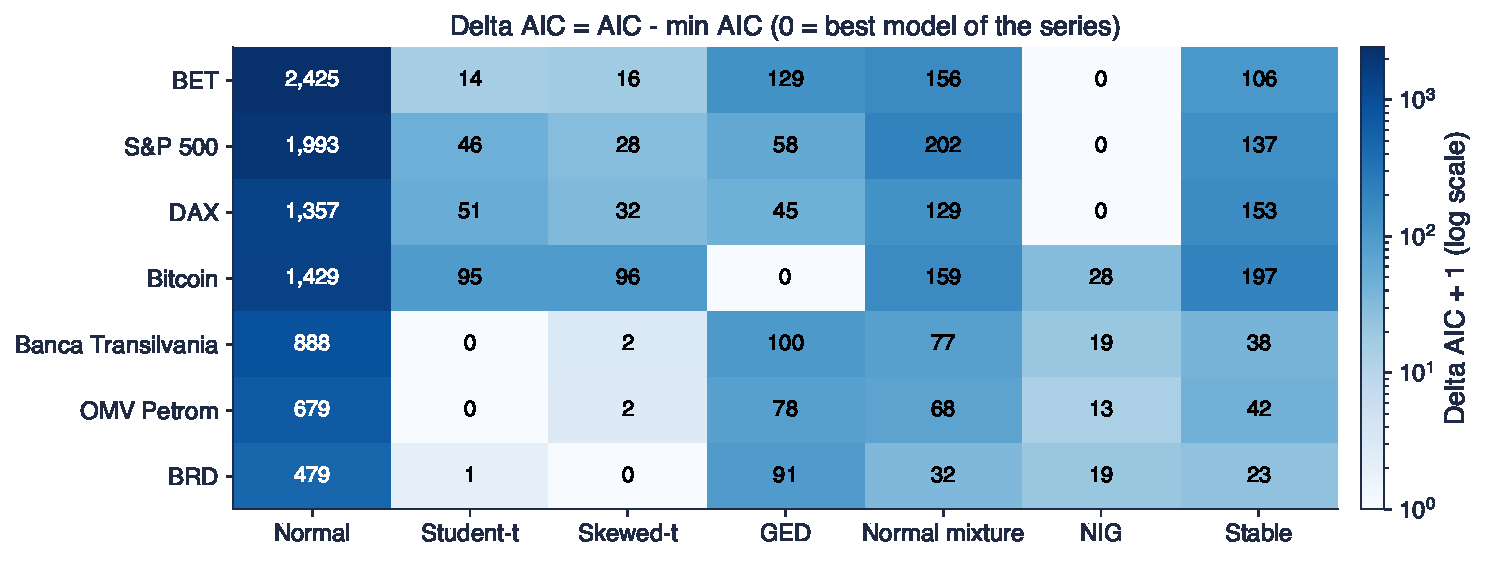
\includegraphics[width=0.97\textwidth,height=0.62\textheight,keepaspectratio]{sfm_ch6_delta_aic.pdf}
\end{center}
\vspace{-0.25cm}
\begin{itemize}
    \item Each row: one series; 0 marks the best model; darker cells: worse models (log colour scale)
\end{itemize}
\quantlet{SFM\_ch6\_lr\_aic}{\qlurl{SFM_ch6_lr_aic}}
\end{frame}

\begin{frame}{Reading the $\Delta$AIC Map}
\itemsize{\small}
\begin{itemize}
    \item No single winner: the best model depends on the market
    \begin{itemize}
        \item indices (BET, S\&P 500, DAX): NIG; Bitcoin: GED; BVB stocks: Student-t (TLV, SNP) and skewed-t (BRD)
    \end{itemize}
    \item Robust conclusions
    \begin{itemize}
        \item the Normal model is last everywhere, by 479 (BRD) to 2\,425 (BET) points
        \item the stable law ($\Delta$ from 23 to 197) and the Normal mixture are never competitive
    \end{itemize}
    \item \textbf{Question for the room}: for BRD, AIC prefers the skewed-t ($\Delta$ of the Student-t: $1.0$); which model does BIC prefer?
    \item \textbf{Answer}
    \begin{itemize}
        \item the Student-t: one parameter less saves $\ln n \approx 8.2$ BIC points, more than the gain in fit; with $\Delta \approx 1$ the two are practically tied
    \end{itemize}
\end{itemize}
\end{frame}

\begin{frame}{Recap: Information Criteria}
\itemsize{\small}
\begin{itemize}
    \item AIC $= -2\ell + 2k$ (prediction); BIC $= -2\ell + k\ln n$ (true model, heavier penalty)
    \item Read $\Delta$AIC and Akaike weights, not the AIC level; $\Delta \le 2$ is a tie
    \item Indices: NIG; Bitcoin: GED; BVB stocks: Student-t; Normal and stable: never
    \item AIC ranks the candidates; it does not say whether the best one is good enough
\end{itemize}
\end{frame}


%=============================================================================
\section{Goodness-of-Fit Tests}
%=============================================================================

\begin{frame}{From Pearson to the Empirical Distribution Function}
\itemsize{\small}
\begin{columns}[T]
\begin{column}{0.64\textwidth}
\begin{itemize}
    \item \refPearson: the first goodness-of-fit test, the $\chi^2$ test
    \begin{itemize}
        \item group the data into bins and compare observed with expected counts
        \item the result depends on the bins, and the tails hold few observations
    \end{itemize}
    \item \textbf{Empirical distribution function} (EDF): $F_n(x) = \frac{1}{n}\#\{t: r_t \le x\}$
    \begin{itemize}
        \item no bins: compare $F_n$ with the model distribution function $F$
    \end{itemize}
    \item Three EDF tests: Kolmogorov--Smirnov, Cramér--von Mises, Anderson--Darling \refStephens
\end{itemize}
\end{column}
\begin{column}{0.32\textwidth}
\centering
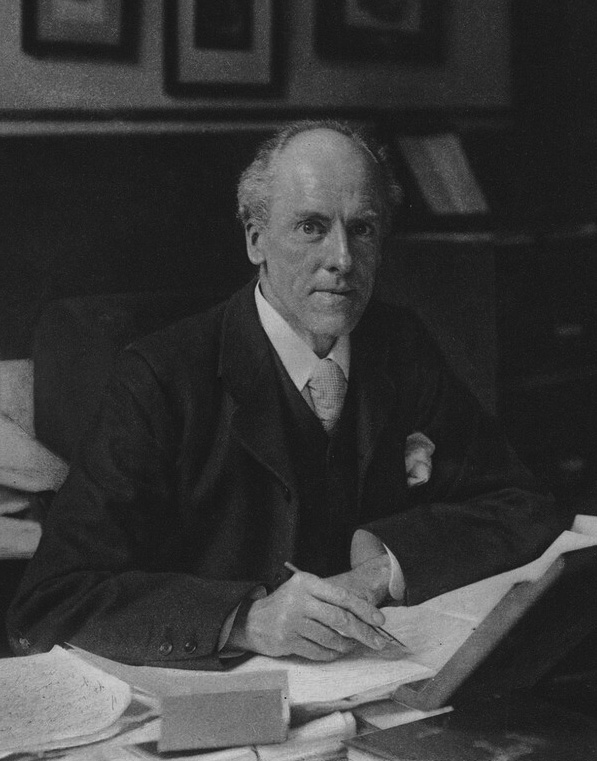
\includegraphics[height=0.44\textheight]{ch6_pearson.jpg}\\[1mm]
\imgcap{Karl Pearson (1857--1936)}
\imgcredit{https://commons.wikimedia.org/wiki/File:Karl_Pearson.jpg}{Photogravure (1910); public domain; Wikimedia Commons}
\end{column}
\end{columns}
\end{frame}

\begin{frame}{The Kolmogorov--Smirnov Test}
\itemsize{\small}
\begin{columns}[T]
\begin{column}{0.6\textwidth}
\begin{itemize}
    \item $D_n = \sup_x |F_n(x) - F(x)|$, the largest vertical gap between the EDF and the model CDF ($\sup$: the largest value over all $x$)
    \begin{itemize}
        \item $r_{(i)}$: the $i$-th smallest return; $u_{(i)} = F(r_{(i)})$: its model probability
        \item computing formula: $D_n = \max_i \max\{i/n - u_{(i)},\ u_{(i)} - (i-1)/n\}$
    \end{itemize}
    \item $F$ fully known: the law of $D_n$ does not depend on $F$ (Kolmogorov, 1933)
    \begin{itemize}
        \item large $n$: reject at 5\% if $D_n > 1.358/\sqrt{n}$; tables for small $n$: \refSmirnov
        \item $n = 6\,714$: critical value $0.017$
    \end{itemize}
    \item Andrey Kolmogorov also gave probability its axioms (\sfmchlink{https://danpele.github.io/SFM/EN/Courses/chapter4_probability.pdf}{Chapter 4})
\end{itemize}
\end{column}
\begin{column}{0.36\textwidth}
\centering
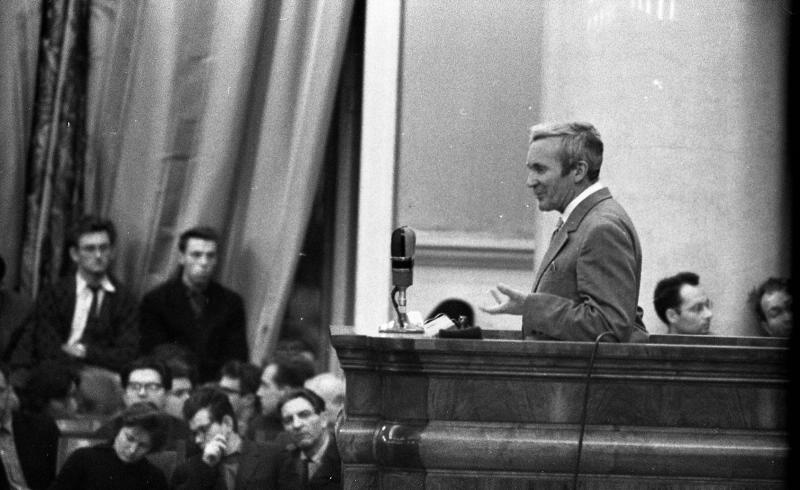
\includegraphics[height=0.38\textheight]{ch4_kolmogorov_1963.jpg}\\[1mm]
\imgcap{Andrey Kolmogorov (1903--1987) lecturing, 1963}
\imgcredit{https://commons.wikimedia.org/wiki/File:Математик_Андрей_Колмогоров_в_аудитории.jpg}{Photo: Vsevolod Tarasevich (1963--1964); CC BY 4.0; Wikimedia Commons}
\end{column}
\end{columns}
\end{frame}

\begin{frame}{Worked Example: KS on Five Returns}
\itemsize{\small}
\begin{itemize}
    \item Returns (\%): $-2.1, -0.4, 0.3, 0.9, 1.6$; $H_0$: $N(0, 1)$, fully specified
    \begin{itemize}
        \item $u_{(i)} = \Phi(r_{(i)})$: $0.018$, $0.345$, $0.618$, $0.816$, $0.945$ ($\Phi$: the standard Normal distribution function)
        \item $i/n$: $0.2, 0.4, 0.6, 0.8, 1.0$; the largest gap is $u_{(3)} - 2/5 = 0.218$
    \end{itemize}
    \item $D_5 = 0.218 < 0.563$, the exact 5\% critical value for $n = 5$: do not reject
    \item With five observations, almost any law passes: the test has little power in small samples
\end{itemize}\quantlet{SFM\_ch6\_gof\_tests}{\qlurl{SFM_ch6_gof_tests}}
\end{frame}

\begin{frame}{Estimated Parameters: the Lilliefors Problem}
\itemsize{\small}
\begin{itemize}
    \item In practice $F$ has estimated parameters: $F(x; \hat\theta)$ is fitted to the same data
    \begin{itemize}
        \item the fit pulls $F$ towards $F_n$: $D_n$ is smaller than under a known $F$
        \item the usual critical values are too large: the test almost never rejects
    \end{itemize}
    \item \refLilliefors: critical values by simulation for the Normal law with $\hat\mu$, $\hat\sigma$ (5\% level)
    \begin{itemize}
        \item $n = 5$: $0.351$ instead of $0.563$; $n = 1000$: $0.029$ instead of $0.043$
    \end{itemize}
    \item Any model: \textbf{parametric bootstrap} \refSGQ
    \begin{itemize}
        \item simulate $n$ draws from $F(\cdot; \hat\theta)$, refit, recompute the statistic; repeat $B$ times
        \item $p$-value $= (1 + \#\{\text{bootstrap statistics} \ge \text{observed}\})/(B + 1)$: the share of simulated statistics at least as large as the observed one
    \end{itemize}
\end{itemize}
\end{frame}

\begin{frame}{Cramér--von Mises and Anderson--Darling}
\itemsize{\small}
\begin{columns}[T]
\begin{column}{0.66\textwidth}
\begin{itemize}
    \item Both integrate the squared gap $[F_n(x) - F(x)]^2$ over all $x$ instead of taking its maximum
    \begin{itemize}
        \item \textbf{Cramér--von Mises}: $W^2 = n\int [F_n - F]^2\, dF = \frac{1}{12n} + \sum_i \big(u_{(i)} - \frac{2i - 1}{2n}\big)^2$ \refCramer
        \item \textbf{Anderson--Darling}: $A^2 = n\int \dfrac{[F_n - F]^2}{F(1 - F)}\, dF$ \refAD
    \end{itemize}
    \item Computing formula \refADb: $A^2 = -n - \frac{1}{n}\sum_i (2i - 1)\big[\ln u_{(i)} + \ln(1 - u_{(n + 1 - i)})\big]$
    \begin{itemize}
        \item $u_{(i)} = F(r_{(i)})$ as in KS; large $W^2$ or $A^2$: a poor fit
        \item the weight $1/[F(1 - F)]$ is huge where $F$ is near 0 or 1: the tails
    \end{itemize}
\end{itemize}
\end{column}
\begin{column}{0.30\textwidth}
\centering
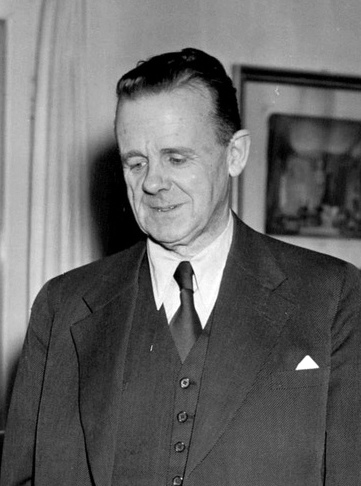
\includegraphics[height=0.42\textheight]{ch6_cramer.jpg}\\[1mm]
\imgcap{Harald Cramér (1893--1985)}
\imgcredit{https://commons.wikimedia.org/wiki/File:Harald_Cramér.jpg}{Photo: unknown photographer (1951); public domain; Wikimedia Commons}
\end{column}
\end{columns}
\end{frame}

\begin{frame}{Why KS Is Weak in the Tails}
\itemsize{\footnotesize}
\begin{center}
    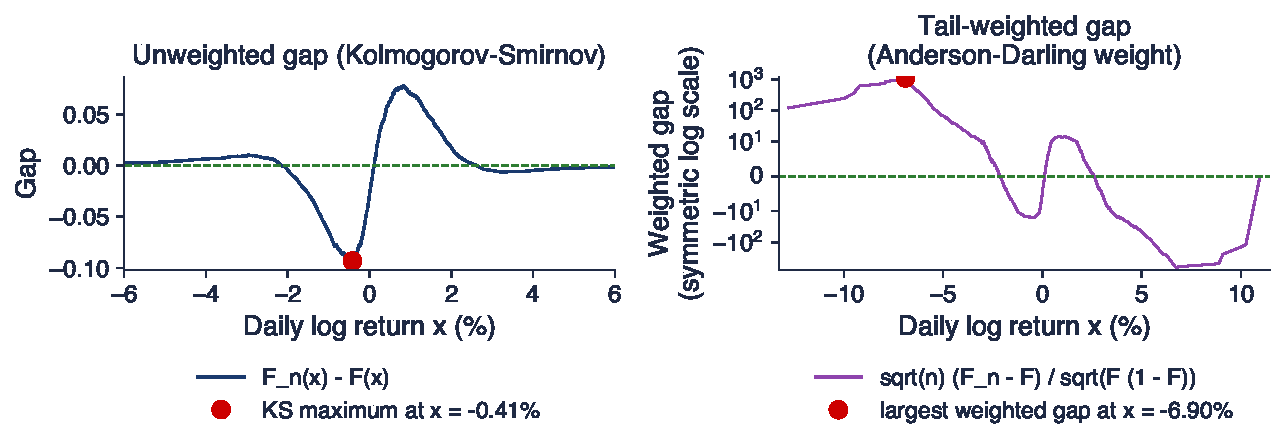
\includegraphics[width=0.97\textwidth,height=0.50\textheight,keepaspectratio]{sfm_ch6_ks_tail.pdf}
\end{center}
\vspace{-0.25cm}
\begin{itemize}
    \item S\&P 500 against its Normal fit. Left: the KS gap peaks at $x = -0.41\%$, near the centre ($F = 36\%$), with $D_n = 0.093$
    \item In the tails $F_n$ and $F$ are both close to 0 or 1, so the raw gap is small even when the model is badly wrong
    \begin{itemize}
        \item the Anderson--Darling weight (right) puts the largest gap at $x = -6.9\%$
    \end{itemize}
\end{itemize}
\quantlet{SFM\_ch6\_gof\_tests}{\qlurl{SFM_ch6_gof_tests}}
\end{frame}

\begin{frame}{Power of the Three Tests}
\itemsize{\footnotesize}
\begin{center}
    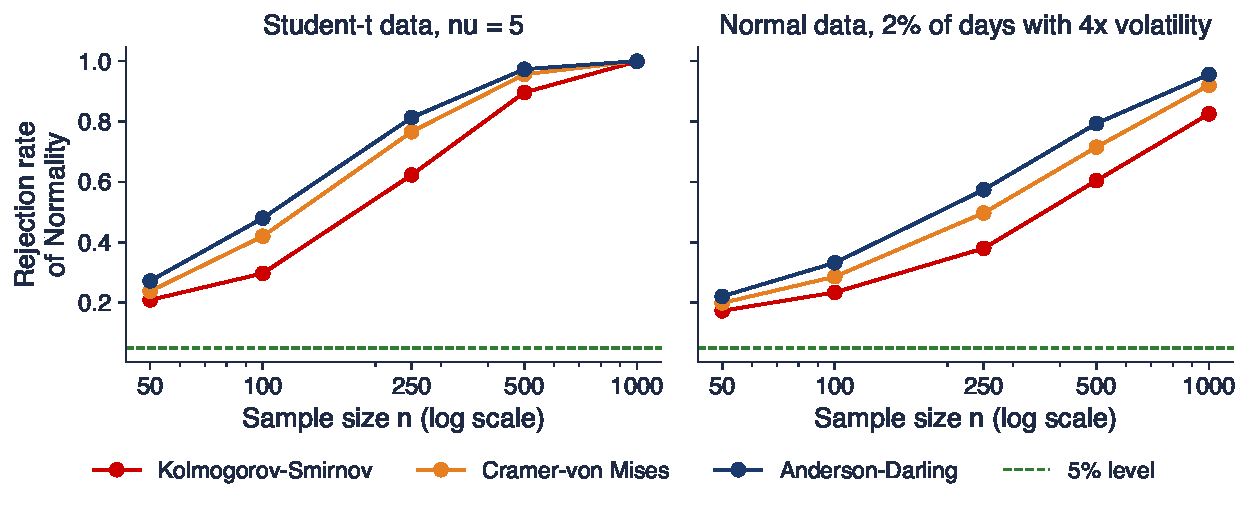
\includegraphics[width=0.97\textwidth,height=0.50\textheight,keepaspectratio]{sfm_ch6_gof_power.pdf}
\end{center}
\vspace{-0.25cm}
\begin{itemize}
    \item Share of 1000 simulated samples in which Normality (estimated parameters) is rejected at 5\%; power = probability of rejecting a false $H_0$
    \item Student-t data, $n = 250$: KS $62\%$, Cramér--von Mises $77\%$, Anderson--Darling $81\%$
    \begin{itemize}
        \item tail-only departures ($n = 250$): $38\%$, $50\%$, $57\%$
    \end{itemize}
\end{itemize}
\quantlet{SFM\_ch6\_gof\_tests}{\qlurl{SFM_ch6_gof_tests}}
\end{frame}

\begin{frame}{EDF Tests on the S\&P 500}
\itemsize{\footnotesize}
\begin{columns}[T]
\begin{column}{0.44\textwidth}
\begin{center}
\scriptsize
\begin{tabular}{lrrr}
\toprule
& KS & CvM & AD \\
\midrule
Normal & $0.093$ & $22.84$ & $127.35$ \\
Student-t & $0.018$ & $0.57$ & $4.69$ \\
skewed-t & $0.017$ & $0.41$ & $2.25$ \\
GED & $0.019$ & $0.38$ & $3.94$ \\
Normal mixture & $0.025$ & $1.09$ & $5.80$ \\
NIG & $0.010$ & $0.13$ & $0.88$ \\
stable & $0.022$ & $0.81$ & $4.61$ \\
\bottomrule
\end{tabular}
\end{center}

\end{column}
\begin{column}{0.52\textwidth}
\begin{itemize}
    \item Parametric bootstrap, $B = 199$, 95\% critical values
    \begin{itemize}
        \item Student-t: KS $0.009$, AD $0.71$
        \item skewed-t: KS $0.008$, AD $0.35$
    \end{itemize}
    \item Normal, Student-t, skewed-t: bootstrap $p = 0.005$, the smallest possible: all rejected
    \item Student-t, naive KS $p$-value (as if $\theta$ were known): $0.021$
\end{itemize}
\end{column}
\end{columns}\begin{itemize}
    \item KS: Kolmogorov--Smirnov; CvM: Cramér--von Mises; AD: Anderson--Darling; smaller is better
\end{itemize}\quantlet{SFM\_ch6\_gof\_tests}{\qlurl{SFM_ch6_gof_tests}}
\end{frame}

\begin{frame}{Statistical vs Practical Significance}
\itemsize{\small}
\begin{itemize}
    \item With $n = 6\,714$ every model is rejected: tests detect tiny departures
    \begin{itemize}
        \item and real returns are not i.i.d.\ (volatility clustering), so no i.i.d.\ law can pass
    \end{itemize}
    \item Use the statistics to \textbf{rank} the models
    \begin{itemize}
        \item AD: Normal $127.35$, Student-t $4.69$, skewed-t $2.25$, NIG $0.88$
        \item as with AIC: NIG first, the Normal model far behind
    \end{itemize}
    \item \textbf{Question for the room}: a KS test on 50 daily returns does not reject the Normal law; is the Normal law then fine for VaR 1\%?
    \item \textbf{Answer}
    \begin{itemize}
        \item no: with $n = 50$ the test rarely rejects even Student-t data ($30\%$ of the time at $n = 100$), and KS barely looks at the tail
    \end{itemize}
\end{itemize}
\end{frame}

\begin{frame}{Recap: Goodness-of-Fit Tests}
\itemsize{\small}
\begin{itemize}
    \item KS: largest gap; CvM: integrated squared gap; AD: the same, weighted towards the tails
    \item Estimated parameters: Lilliefors tables or a parametric bootstrap; never the textbook KS table
    \item Power: AD > CvM > KS for heavy-tailed alternatives
    \item Large samples reject everything: rank by the statistic and look at the plots
\end{itemize}
\end{frame}


%=============================================================================
\section{PP and QQ Plots}
%=============================================================================

\begin{frame}{Two Ways to Look at a Fit}
\itemsize{\small}
\begin{itemize}
    \item \textbf{PP plot} (probability--probability): points $\big(p_i, F(r_{(i)})\big)$ with $p_i = (i - 0.5)/n$
    \begin{itemize}
        \item both axes in $[0, 1]$: differences in the centre show; the tails are squeezed into the corners
        \item the visual twin of KS: the largest vertical distance to the diagonal is close to $D_n$
    \end{itemize}
    \item \textbf{QQ plot} (quantile--quantile): points $\big(F^{-1}(p_i), r_{(i)}\big)$
    \begin{itemize}
        \item in units of returns: the tails are stretched out, each extreme day is visible
        \item ends above/below the line: the model tails are too short; ends flattened: the model tails are too long
    \end{itemize}
    \item Risk management reads QQ plots; PP plots and KS share the same blind spot
\end{itemize}
\end{frame}

\begin{frame}{PP Plots: S\&P 500}
\itemsize{\footnotesize}
\begin{center}
    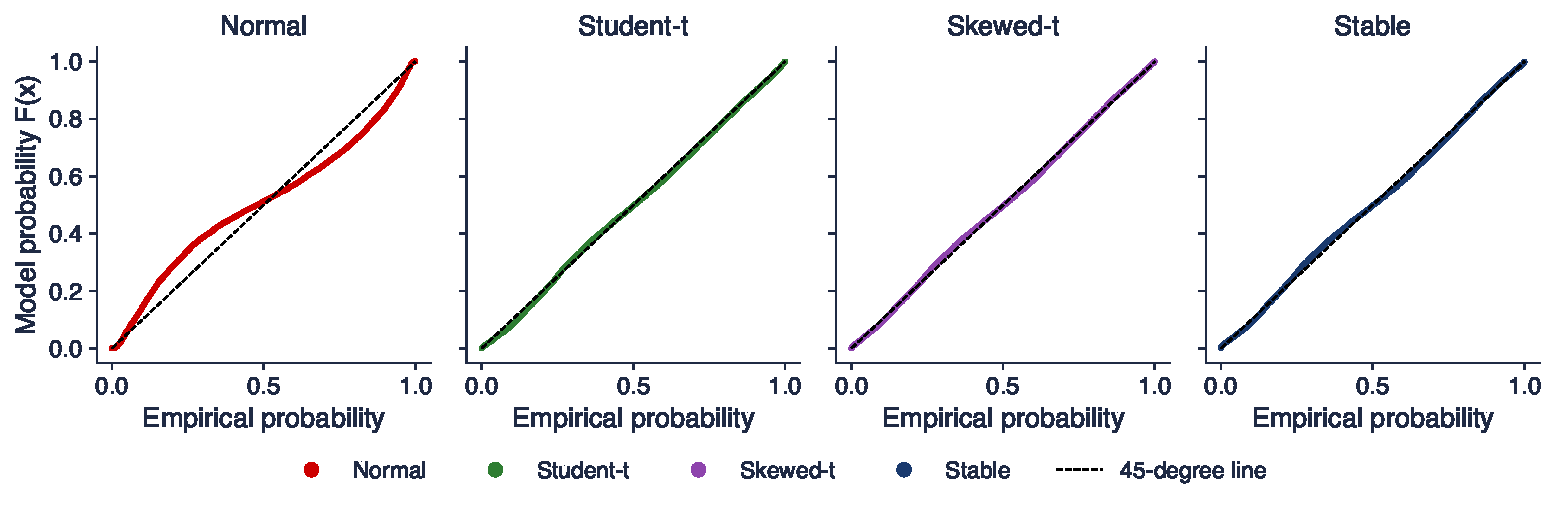
\includegraphics[width=0.97\textwidth,height=0.5\textheight,keepaspectratio]{sfm_ch6_pp.pdf}
\end{center}
\vspace{-0.25cm}
\begin{itemize}
    \item Normal: an S-shape in the centre (too few small returns, too many medium ones), largest gap $0.093$
    \item Student-t, skewed-t, stable: on the diagonal; in a PP plot they are indistinguishable
\end{itemize}
\quantlet{SFM\_ch6\_pp\_qq}{\qlurl{SFM_ch6_pp_qq}}
\end{frame}

\begin{frame}{QQ Plots: S\&P 500}
\itemsize{\footnotesize}
\begin{center}
    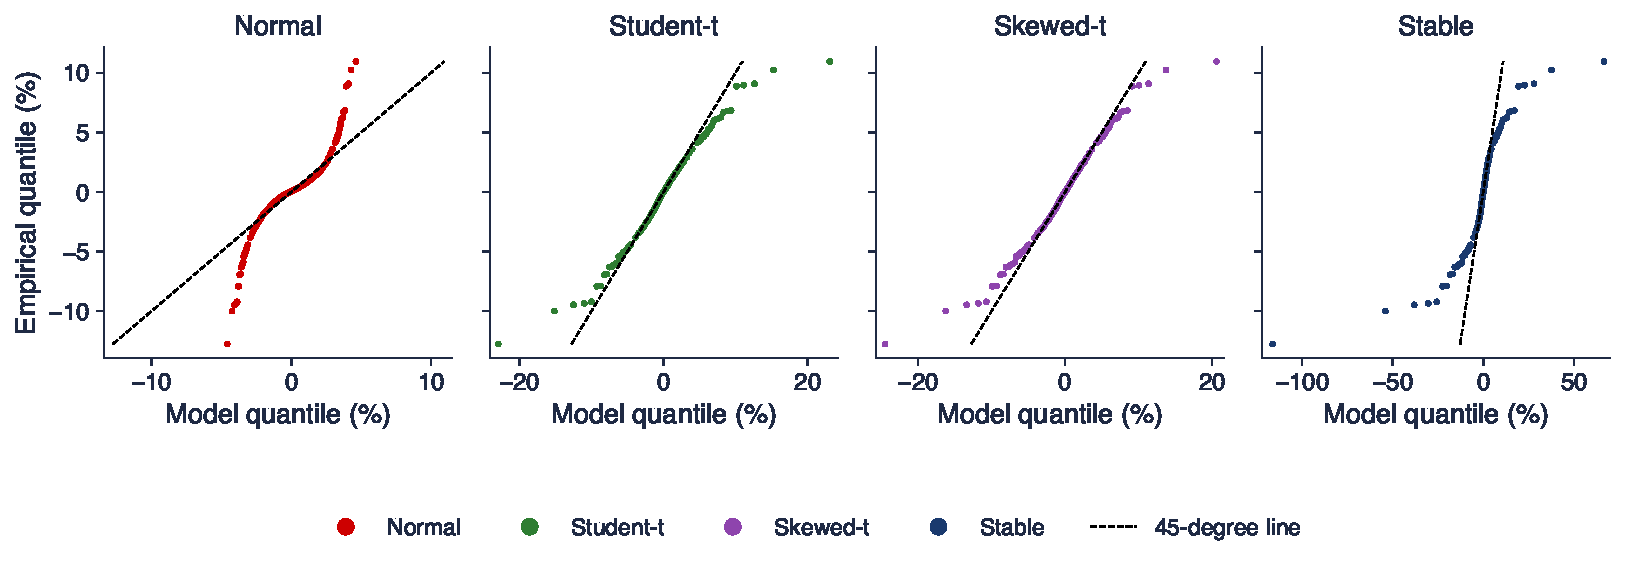
\includegraphics[width=0.97\textwidth,height=0.5\textheight,keepaspectratio]{sfm_ch6_qq.pdf}
\end{center}
\vspace{-0.25cm}
\begin{itemize}
    \item The worst day was $-12.8\%$; the model quantile at the same probability:
    \begin{itemize}
        \item Normal $-4.6\%$, Student-t $-22.9\%$, skewed-t $-24.5\%$, stable $-116.1\%$
    \end{itemize}
    \item The models that looked identical in the PP plot are far apart in the far tail
\end{itemize}
\quantlet{SFM\_ch6\_pp\_qq}{\qlurl{SFM_ch6_pp_qq}}
\end{frame}

\begin{frame}{QQ Plots for BET, Bitcoin and Banca Transilvania}
\itemsize{\footnotesize}
\begin{center}
    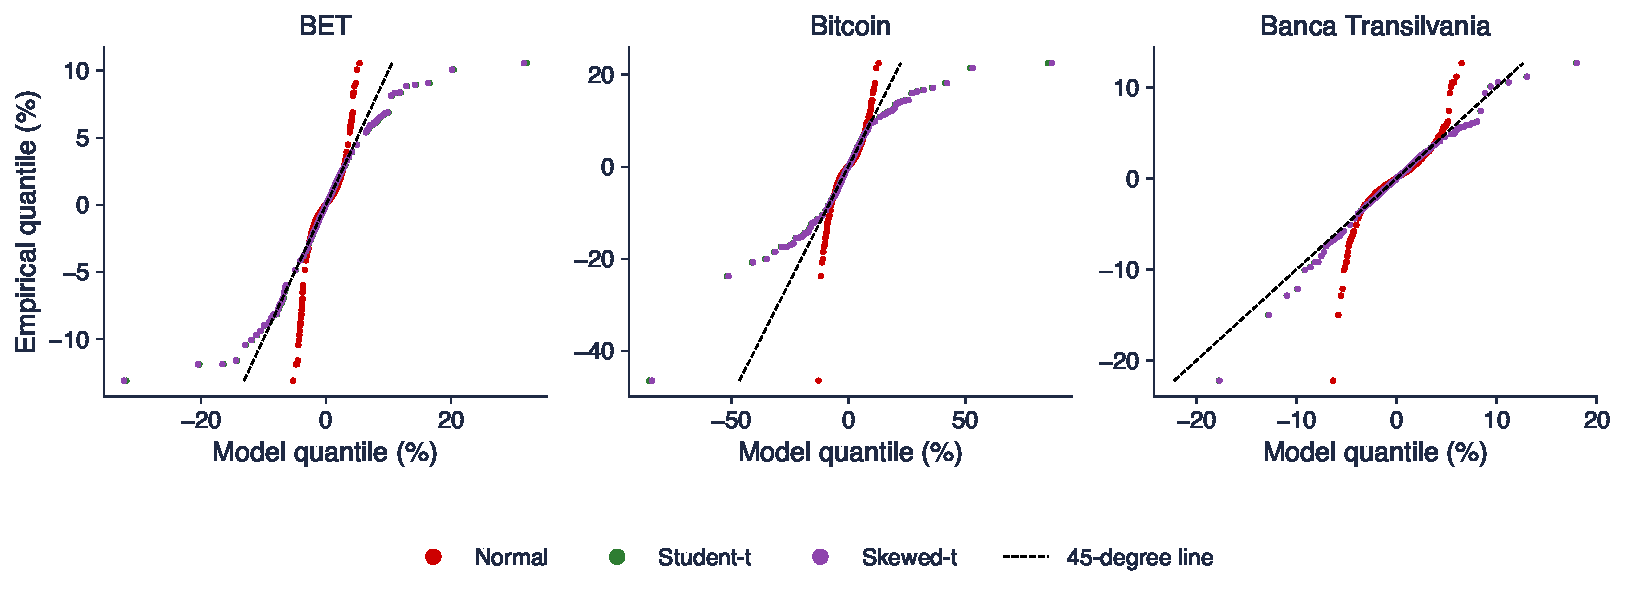
\includegraphics[width=0.97\textwidth,height=0.54\textheight,keepaspectratio]{sfm_ch6_qq_assets.pdf}
\end{center}
\vspace{-0.25cm}
\begin{itemize}
    \item Normal (red): the steep ends of all three series; the Student-t and skewed-t follow the data far into the tails
    \item The last few points are single days (the largest crashes): there the fitted tails disagree most and the uncertainty is widest
\end{itemize}
\quantlet{SFM\_ch6\_pp\_qq}{\qlurl{SFM_ch6_pp_qq}}
\end{frame}

\begin{frame}{Recap: PP and QQ Plots}
\itemsize{\small}
\begin{itemize}
    \item PP: probabilities, good for the centre; QQ: quantiles, good for the tails
    \item Heavy-tailed models that look the same in PP plots differ widely in QQ plots
    \item Always show the QQ plot of the chosen model next to its AIC
\end{itemize}
\end{frame}


%=============================================================================
\section{The Purpose Decides: Which Model Gets VaR 1\% Right?}
%=============================================================================

\begin{frame}{VaR and ES}
\itemsize{\small}
\begin{itemize}
    \item Return $X$, level $\alpha$ (here $\alpha = 1\%$ or $2.5\%$, the probability of the tail)
    \begin{itemize}
        \item \textbf{VaR} (Value at Risk): $\mathrm{VaR}_\alpha = -q_\alpha(X)$, the loss exceeded with probability $\alpha$
        \item \textbf{ES} (expected shortfall): $\mathrm{ES}_\alpha = -\frac{1}{\alpha}\int_0^\alpha q_u\, du = -E[X \mid X \le q_\alpha]$, the average loss in the tail
    \end{itemize}
    \item Normal model: $\mathrm{VaR}_\alpha = -(\mu + \sigma z_\alpha)$, $z_{0.01} = -2.326$
    \begin{itemize}
        \item S\&P 500: $-(0.025 - 2.326 \times 1.213) = 2.80\%$, against the empirical VaR 1\% of $3.45\%$
    \end{itemize}
    \item Basel rules: ES 2.5\% for market risk, VaR 1\% for backtesting (\sfmchlink{https://danpele.github.io/SFM/EN/Courses/chapter10_var_es_backtesting.pdf}{Chapter 10})
\end{itemize}
\end{frame}

\begin{frame}{VaR 1\% and ES 2.5\% under Each Model (In Sample)}
\itemsize{\footnotesize}
\textbf{VaR 1\%} (\%)\begin{center}
\scriptsize
\begin{tabular}{lrrrrrrr}
\toprule
& data & Normal & Student-t & skewed-t & GED & NIG & stable \\
\midrule
BET & $4.13$ & $3.19$ & $4.06$ & $4.10$ & $3.74$ & $4.11$ & $4.94$ \\
S\&P 500 & $3.45$ & $2.80$ & $3.46$ & $3.71$ & $3.27$ & $3.72$ & $4.54$ \\
DAX & $4.16$ & $3.25$ & $3.96$ & $4.24$ & $3.77$ & $4.24$ & $5.01$ \\
Bitcoin & $10.51$ & $7.99$ & $11.06$ & $10.91$ & $9.85$ & $10.52$ & $14.26$ \\
TLV & $5.10$ & $4.01$ & $4.63$ & $4.61$ & $4.49$ & $4.76$ & $4.92$ \\
SNP & $4.29$ & $3.70$ & $4.26$ & $4.22$ & $4.16$ & $4.32$ & $4.43$ \\
BRD & $4.50$ & $3.81$ & $4.24$ & $4.39$ & $4.18$ & $4.43$ & $4.51$ \\
\bottomrule
\end{tabular}
\end{center}
\textbf{ES 2.5\%} (\%)\begin{center}
\scriptsize
\begin{tabular}{lrrrrrrr}
\toprule
& data & Normal & Student-t & skewed-t & GED & NIG & stable \\
\midrule
BET & $4.57$ & $3.21$ & $4.76$ & $4.81$ & $3.85$ & $4.31$ & $7.58$ \\
S\&P 500 & $3.76$ & $2.81$ & $3.95$ & $4.23$ & $3.36$ & $3.89$ & $6.70$ \\
Bitcoin & $10.84$ & $8.03$ & $13.37$ & $13.18$ & $10.17$ & $11.06$ & $22.87$ \\
\bottomrule
\end{tabular}
\end{center}
\quantlet{SFM\_ch6\_tail\_var}{\qlurl{SFM_ch6_tail_var}}
\end{frame}

\begin{frame}{Model VaR 1\% Relative to the Data}
\itemsize{\footnotesize}
\begin{center}
    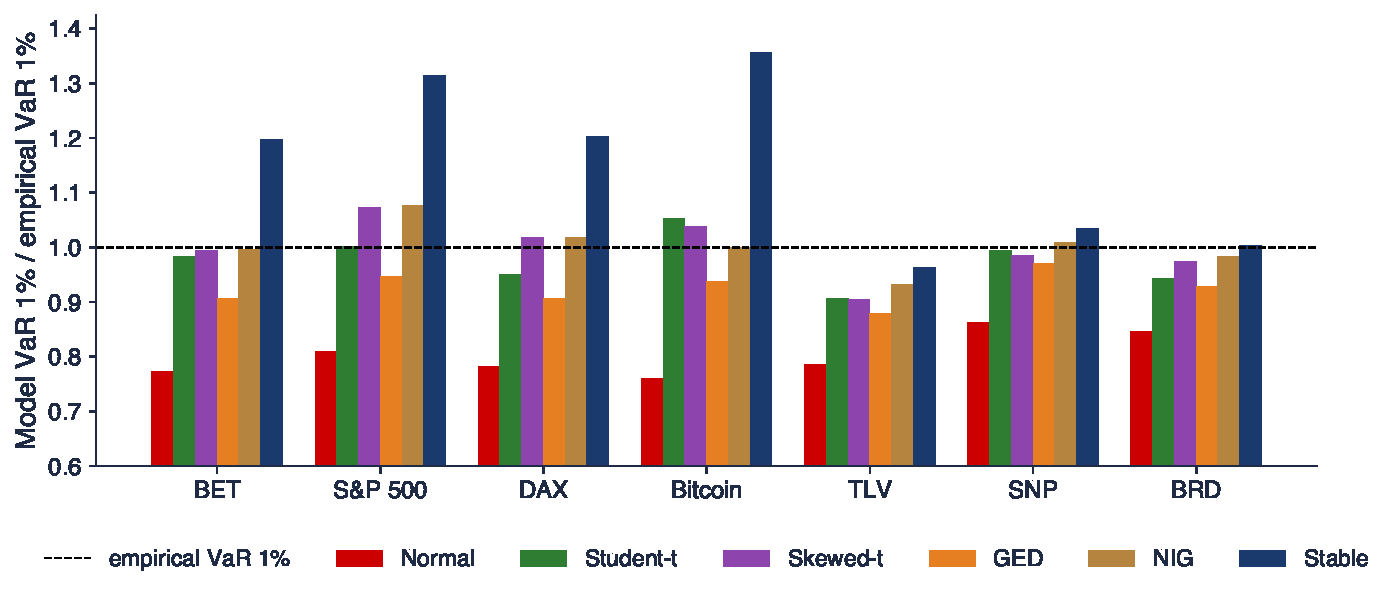
\includegraphics[width=0.97\textwidth,height=0.55\textheight,keepaspectratio]{sfm_ch6_var_models.pdf}
\end{center}
\vspace{-0.25cm}
\begin{itemize}
    \item Normal: $14$--$24\%$ too low everywhere; stable: up to $36\%$ too high
    \item Student-t, skewed-t and NIG stay within $10\%$ of the empirical VaR 1\%; GED is a little low
\end{itemize}
\quantlet{SFM\_ch6\_tail\_var}{\qlurl{SFM_ch6_tail_var}}
\end{frame}

\begin{frame}{The Left Tail on Log-Log Axes (S\&P 500)}
\itemsize{\footnotesize}
\begin{center}
    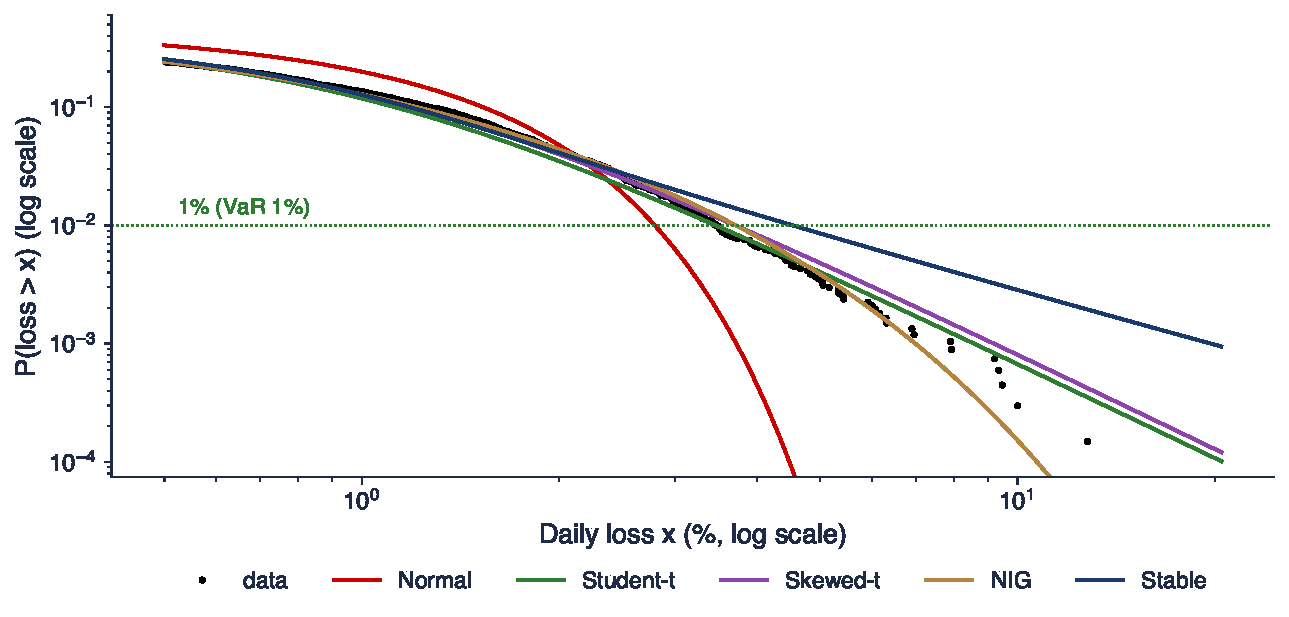
\includegraphics[width=0.97\textwidth,height=0.58\textheight,keepaspectratio]{sfm_ch6_left_tail.pdf}
\end{center}
\vspace{-0.25cm}
\begin{itemize}
    \item Points: share of days with a loss above $x$; lines: the same probability under each fitted model
    \item At 1\% all heavy-tailed models are close; beyond $5\%$ losses the stable line is far too high and the Normal one collapses
\end{itemize}
\quantlet{SFM\_ch6\_tail\_var}{\qlurl{SFM_ch6_tail_var}}
\end{frame}

\begin{frame}{Counting Exceedances: the Kupiec Test}
\itemsize{\footnotesize}
\begin{center}
\scriptsize
\begin{tabular}{lrrrrrrr}
\toprule
& expected & Normal & Student-t & skewed-t & GED & NIG & stable \\
\midrule
BET & 67 & 138 & 71 & 69 & 91 & 68 & 43 \\
S\&P 500 & 67 & 131 & 67 & 52 & 80 & 52 & 30 \\
DAX & 68 & 145 & 78 & 66 & 91 & 65 & 39 \\
Bitcoin & 44 & 86 & 34 & 36 & 56 & 44 & 16 \\
\bottomrule
\end{tabular}
\end{center}
\begin{itemize}
    \item Exceedance: a day with $r_t < -\mathrm{VaR}_{1\%}$; under a correct model their number is $\mathrm{Binomial}(n, 0.01)$
    \item \refKupiec: $LR_{uc} = -2\ln\dfrac{(1-\alpha)^{n - x}\alpha^x}{(1 - x/n)^{n - x}(x/n)^x} \approx \chi^2(1)$, $x$ = number of exceedances
    \begin{itemize}
        \item an LR test comparing the target rate $\alpha$ with the observed rate $x/n$; large $LR_{uc}$: wrong number of exceedances
    \end{itemize}
    \item S\&P 500: Student-t 67 exceedances for 67 expected ($p = 0.986$)
    \begin{itemize}
        \item NIG, the AIC winner, 52 ($p = 0.053$)
    \end{itemize}
    \item The best model for the whole density is not always the best for one quantile; tail-focused scores exist \refDPD
\end{itemize}\quantlet{SFM\_ch6\_tail\_var}{\qlurl{SFM_ch6_tail_var}}
\end{frame}

\begin{frame}{Recap: VaR 1\% in Sample}
\itemsize{\small}
\begin{itemize}
    \item VaR 1\% $= -q_{1\%}$, ES 2.5\% = average loss beyond $q_{2.5\%}$
    \item Normal: VaR 1\% $14$--$24\%$ too low; stable: much too high; Student-t, skewed-t, NIG: close
    \item Judge a risk model by its exceedances (Kupiec), not only by AIC
\end{itemize}
\end{frame}


%=============================================================================
\section{Out of Sample: Validation and Overfitting}
%=============================================================================

\begin{frame}{Why Out of Sample?}
\itemsize{\small}
\begin{itemize}
    \item In sample, a larger model always fits at least as well: $\ell$ never decreases when parameters are added
    \begin{itemize}
        \item \textbf{overfitting}: the extra parameters fit noise of the estimation sample, not features of future returns
    \end{itemize}
    \item The honest check: estimate until 31 December 2019, evaluate on 2020--2026 (COVID-19 crash, 2022 inflation shock, 2025 tariffs)
    \begin{itemize}
        \item \textbf{log score}: the mean of $\ln f(r_t; \hat\theta)$ over the test days; higher is better, a proper scoring rule \refGR
        \item \textbf{exceedances} of VaR 1\% (Kupiec) and the \textbf{pinball loss} $\frac{1}{n}\sum_t (\alpha - \mathbf{1}\{r_t < q\})(r_t - q)$ of the 1\% quantile $q$
        \item pinball: $\mathbf{1}\{r_t < q\} = 1$ on a day below $q$, 0 otherwise; it penalises misses asymmetrically, lower is better
    \end{itemize}
    \item A score is \textbf{proper} if the true distribution gets the best expected score: forecasters cannot gain by distorting
\end{itemize}
\end{frame}

\begin{frame}{Out-of-Sample Results, 2020--2026}
\itemsize{\footnotesize}
\begin{center}
    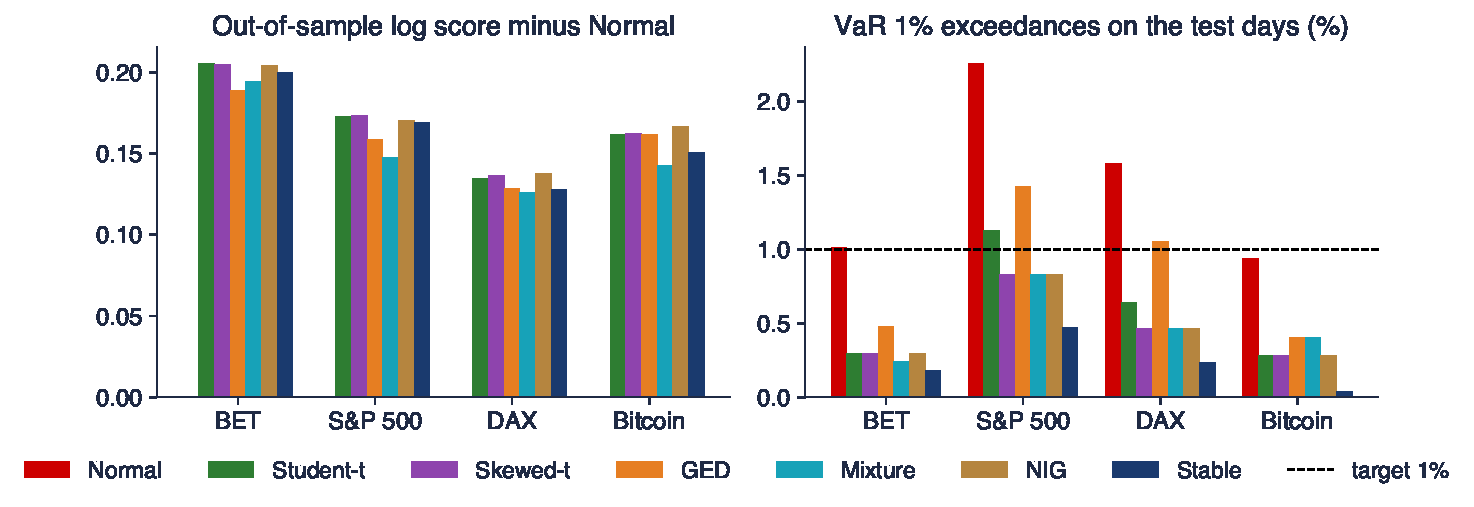
\includegraphics[width=0.97\textwidth,height=0.55\textheight,keepaspectratio]{sfm_ch6_oos.pdf}
\end{center}
\vspace{-0.25cm}
\begin{itemize}
    \item Left: every heavy-tailed model beats the Normal log score by $0.13$ to $0.21$ per day; the differences among them are small
    \item Right: VaR 1\% exceedance rates; the target is the dashed line at 1\%
\end{itemize}
\quantlet{SFM\_ch6\_out\_of\_sample}{\qlurl{SFM_ch6_out_of_sample}}
\end{frame}

\begin{frame}{Reading the Out-of-Sample Table}
\itemsize{\footnotesize}
\begin{center}
\scriptsize
\begin{tabular}{lrrrrrrrll}
\toprule
& exp. & Normal & t & skew-t & NIG & stable & hist. & best AIC & best log score \\
\midrule
BET & 16.7 & 17 & 5 & 5 & 5 & 3 & 5 & NIG & Student-t \\
S\&P 500 & 16.9 & 38 & 19 & 14 & 14 & 8 & 23 & NIG & skewed-t \\
DAX & 17.1 & 27 & 11 & 8 & 8 & 4 & 8 & NIG & NIG \\
Bitcoin & 24.5 & 23 & 7 & 7 & 7 & 1 & 10 & GED & NIG \\
\bottomrule
\end{tabular}
\end{center}
\begin{itemize}
    \item VaR 1\% exceedances on the test days; exp.: expected number; hist.: historical simulation (the 1\% quantile of the estimation sample)
    \item The AIC winner of 2000--2019 has the best log score only for the DAX; elsewhere the best log score belongs to a close neighbour
    \item BET: the Normal model has 17 exceedances for 16.7 expected, the heavy-tailed models only 5
    \begin{itemize}
        \item 2020--2026 was calmer for the BET than 2000--2019
    \end{itemize}
    \item The right count for the wrong reason: a static model cannot follow changes in volatility
\end{itemize}\quantlet{SFM\_ch6\_out\_of\_sample}{\qlurl{SFM_ch6_out_of_sample}}
\end{frame}

\begin{frame}{Overfitting: Normal Mixtures with 1 to 6 Components}
\itemsize{\footnotesize}
\begin{center}
    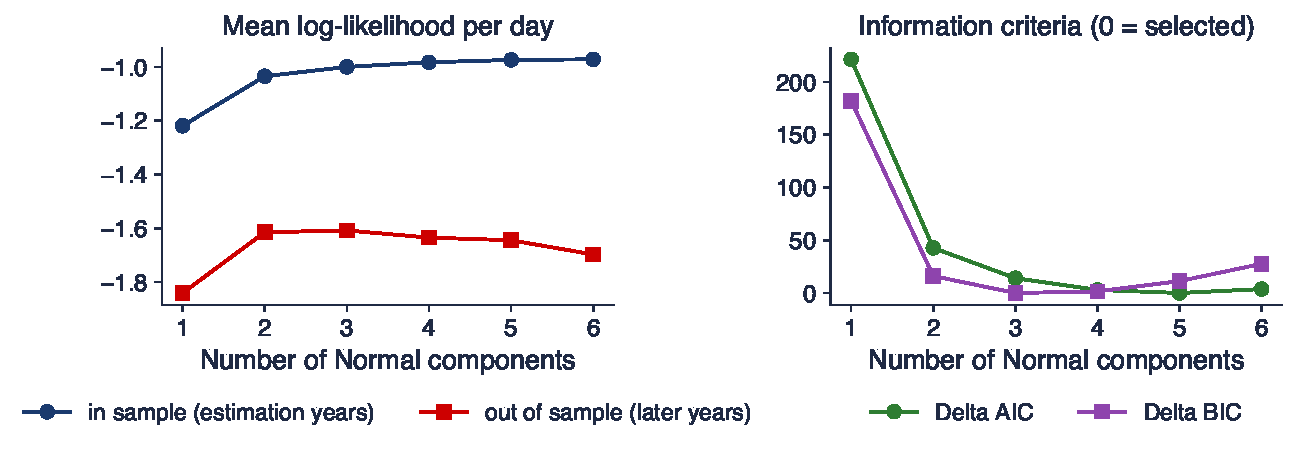
\includegraphics[width=0.97\textwidth,height=0.52\textheight,keepaspectratio]{sfm_ch6_overfit.pdf}
\end{center}
\vspace{-0.25cm}
\begin{itemize}
    \item S\&P 500, estimation 2017--2018 ($n = 501$), test 2019--2026 ($n = 1\,939$); $c$ components have $3c - 1$ parameters
    \item In sample (blue) the fit improves with every component; out of sample (red) it peaks at $c = 3$ and then declines
\end{itemize}
\quantlet{SFM\_ch6\_out\_of\_sample}{\qlurl{SFM_ch6_out_of_sample}}
\end{frame}

\begin{frame}{Which Criterion Warned Us?}
\itemsize{\small}
\begin{itemize}
    \item Mean log-likelihood per day, in sample $\to$ out of sample
    \begin{itemize}
        \item $c = 1$ (Normal): $-1.219 \to -1.841$; $c = 3$: $-0.999 \to -1.608$; $c = 6$ (17 parameters): $-0.971 \to -1.698$
    \end{itemize}
    \item BIC chose $c = 3$, the best model out of sample; AIC chose $c = 5$
    \begin{itemize}
        \item with $n = 501$, AIC's penalty of 2 per parameter is too weak to stop extra components
    \end{itemize}
    \item The gap between in-sample and out-of-sample fit grows with the number of parameters: that gap is the overfitting
    \item Rule: short samples, many parameters $\Rightarrow$ prefer BIC or AICc, and always keep a test period
\end{itemize}\quantlet{SFM\_ch6\_out\_of\_sample}{\qlurl{SFM_ch6_out_of_sample}}
\end{frame}

\begin{frame}{Rolling VaR 1\%: Refit Every Month}
\itemsize{\footnotesize}
\begin{center}
    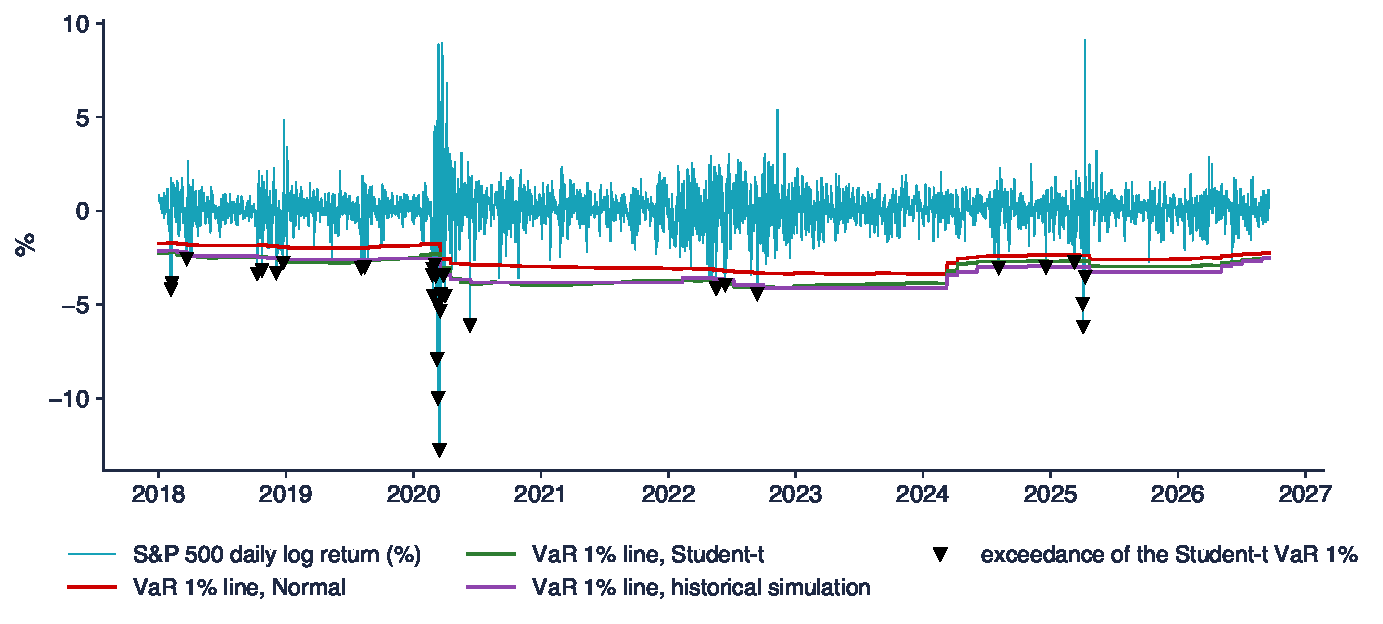
\includegraphics[width=0.97\textwidth,height=0.55\textheight,keepaspectratio]{sfm_ch6_rolling_var.pdf}
\end{center}
\vspace{-0.25cm}
\begin{itemize}
    \item S\&P 500: each model refitted every 20 trading days on the previous 1000 days; the VaR 1\% line is drawn as a loss threshold $-\mathrm{VaR}$
    \item Black triangles: exceedances of the Student-t VaR; they come in clusters (March 2020)
\end{itemize}
\quantlet{SFM\_ch6\_out\_of\_sample}{\qlurl{SFM_ch6_out_of_sample}}
\end{frame}

\begin{frame}{Rolling Backtest: the Results}
\itemsize{\footnotesize}
\begin{center}
\footnotesize
\begin{tabular}{lrrrr}
\toprule
& Normal & Student-t & skewed-t & historical \\
\midrule
S\&P 500, rate (\%) & $2.35$ & $1.56$ & $1.47$ & $1.58$ \\
S\&P 500, Kupiec $p$ & $<0.001$ & $<0.001$ & $<0.001$ & $<0.001$ \\
S\&P 500, most in one year & 36 & 31 & 28 & 29 \\
BET, rate (\%) & $1.98$ & $1.52$ & $1.38$ & $1.25$ \\
BET, Kupiec $p$ & $<0.001$ & $<0.001$ & $0.007$ & $0.066$ \\
\bottomrule
\end{tabular}
\end{center}
\begin{itemize}
    \item Backtest 2003--2026, $n = 5\,714$ days for the S\&P 500; target rate 1\%; the worst year is 2008 for every model and both series
    \item Heavy tails halve the excess of exceedances, but no unconditional model reaches 1\%
    \begin{itemize}
        \item the volatility changes faster than a 1000-day window can adapt
    \end{itemize}
    \item The remedy is a model for the volatility itself: GARCH, \sfmchlink{https://danpele.github.io/SFM/EN/Courses/chapter8_volatility_estimators.pdf}{Chapters 8} and \sfmchlink{https://danpele.github.io/SFM/EN/Courses/chapter9_arch_garch_models.pdf}{9}
\end{itemize}\quantlet{SFM\_ch6\_out\_of\_sample}{\qlurl{SFM_ch6_out_of_sample}}
\end{frame}

\begin{frame}{The VaR Reliability Plot (SFEVaRqqplot)}
\itemsize{\scriptsize}
\begin{center}
    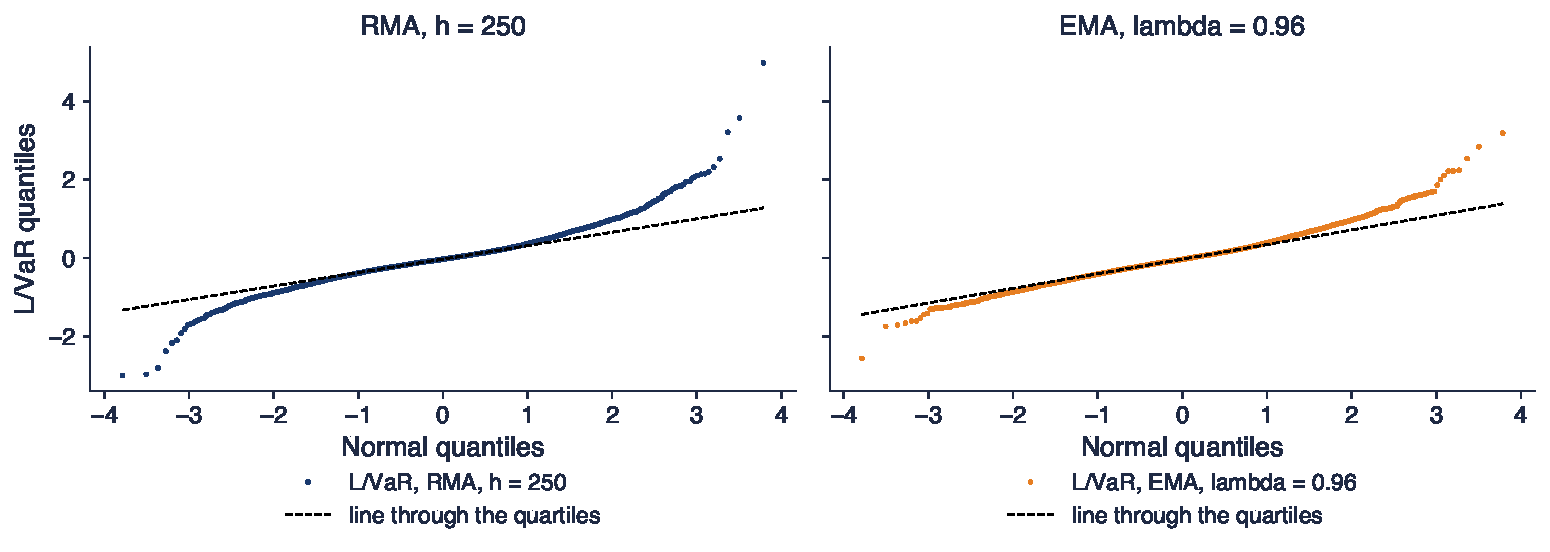
\includegraphics[width=0.97\textwidth,height=0.46\textheight,keepaspectratio]{sfm_ch6_var_qqplot.pdf}
\end{center}
\vspace{-0.25cm}
\begin{itemize}
    \item DAX since 2000: Normal VaR 1\% $= -z_{0.01}\hat\sigma_t = 2.326\,\hat\sigma_t$, with $\hat\sigma_t$ from the previous 250 days
    \begin{itemize}
        \item RMA (rectangular moving average): $\hat\sigma_t^2 = \frac{1}{250}\sum_{j=1}^{250} r_{t-j}^2$, equal weights
        \item EMA (exponential moving average): $\hat\sigma_t^2 = (1 - \lambda)\sum_{j \ge 0} \lambda^j r_{t-1-j}^2$, $\lambda = 0.96$: each older day weighs 4\% less
        \item QQ plot of $L/\mathrm{VaR}$ (loss divided by VaR) against Normal quantiles
    \end{itemize}
    \item A straight line would mean a reliable VaR; both curve upwards at the right end
    \begin{itemize}
        \item the losses beyond VaR are too large and too frequent ($2.13\%$ and $2.07\%$ exceedances)
    \end{itemize}
\end{itemize}
\quantlet{SFM\_ch6\_var\_qqplot}{\qlurl{SFM_ch6_var_qqplot}}
\end{frame}

\begin{frame}{Recap: Out of Sample}
\itemsize{\small}
\begin{itemize}
    \item Judge models on data they have not seen: log score, exceedances, pinball loss
    \item Overfitting: in-sample fit rises with parameters, out-of-sample fit does not; BIC protected us, AIC did not
    \item Heavy tails help, but static models fail in crises: volatility must be modelled (GARCH)
\end{itemize}
\end{frame}


%=============================================================================
\section{Model Uncertainty}
%=============================================================================

\begin{frame}{How Sure Are We of the Winner?}
\itemsize{\footnotesize}
\begin{center}
    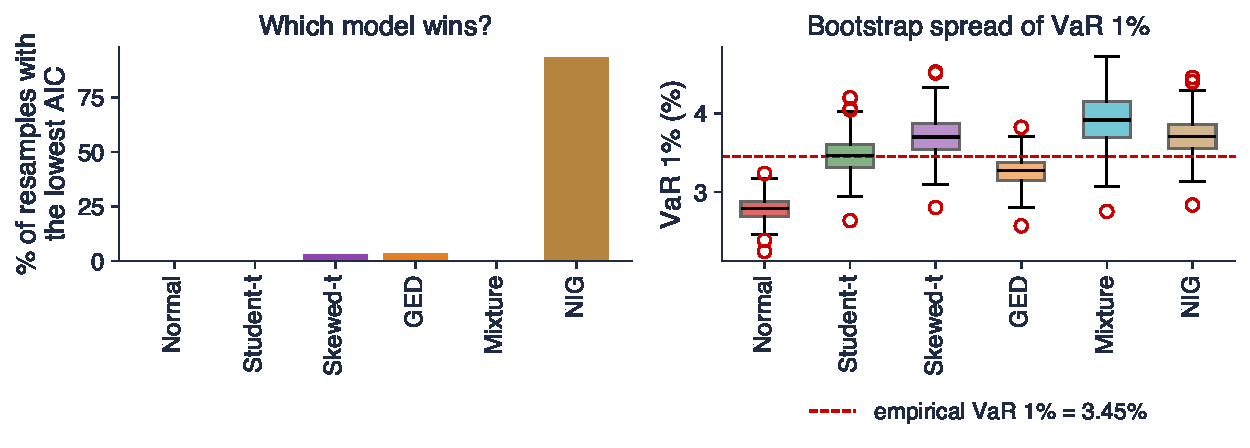
\includegraphics[width=0.97\textwidth,height=0.52\textheight,keepaspectratio]{sfm_ch6_model_uncertainty.pdf}
\end{center}
\vspace{-0.25cm}
\begin{itemize}
    \item S\&P 500, 200 moving-block bootstrap resamples (blocks of 20 days keep the volatility clusters); in each, six models refitted
    \item Left: NIG has the lowest AIC in $94\%$ of the resamples; right: the bootstrap spread of VaR 1\% under each model
\end{itemize}
\quantlet{SFM\_ch6\_model\_uncertainty}{\qlurl{SFM_ch6_model_uncertainty}}
\end{frame}

\begin{frame}{Two Sources of Uncertainty}
\itemsize{\small}
\begin{itemize}
    \item \textbf{Parameter uncertainty}: the same model, re-estimated on resampled data
    \begin{itemize}
        \item Student-t VaR 1\%: 90\% bootstrap band $[3.14, 3.87]\%$; NIG: $[3.34, 4.18]\%$
    \end{itemize}
    \item \textbf{Model uncertainty}: different models on the same data
    \begin{itemize}
        \item median VaR 1\%: GED $3.27\%$, Student-t $3.47\%$, NIG $3.71\%$, Normal mixture $3.92\%$
        \item the spread between models is comparable to the spread within one model
    \end{itemize}
    \item Even when the AIC winner is clear, the number that matters for risk is not
    \item Entropy-based tail measures are another way to summarise this uncertainty: \refPeleA, \refPeleB
\end{itemize}
\end{frame}

\begin{frame}{Model Averaging and Model Risk}
\itemsize{\footnotesize}
\begin{center}
\scriptsize
\begin{tabular}{lrrrrr}
\toprule
& data & Normal & heavy-tailed range & averaged & range (\%) \\
\midrule
BET & $4.13$ & $3.19$ & $[3.74, 4.94]$ & $4.11$ & $32$ \\
S\&P 500 & $3.45$ & $2.80$ & $[3.27, 4.54]$ & $3.72$ & $39$ \\
DAX & $4.16$ & $3.25$ & $[3.77, 5.01]$ & $4.24$ & $33$ \\
Bitcoin & $10.51$ & $7.99$ & $[9.85, 14.26]$ & $9.85$ & $45$ \\
TLV & $5.10$ & $4.01$ & $[4.49, 5.41]$ & $4.62$ & $21$ \\
SNP & $4.29$ & $3.70$ & $[4.16, 4.70]$ & $4.25$ & $13$ \\
BRD & $4.50$ & $3.81$ & $[4.18, 4.74]$ & $4.33$ & $14$ \\
\bottomrule
\end{tabular}
\end{center}
\begin{itemize}
    \item VaR 1\% in \%; heavy-tailed range: the smallest and largest VaR 1\% of the six non-Normal models
    \begin{itemize}
        \item range (\%): max/min $- 1$, the relative distance between the extreme models
    \end{itemize}
    \item Averaged: $\sum_i w_i\,\mathrm{VaR}_i$ with the Akaike weights $w_i$
    \begin{itemize}
        \item a frequentist cousin of Bayesian model averaging \refHoeting
    \end{itemize}
    \item \textbf{Model risk}: the range across plausible models; regulators ask banks to measure it \refKerkhof, \refDanielsson
\end{itemize}\quantlet{SFM\_ch6\_model\_uncertainty}{\qlurl{SFM_ch6_model_uncertainty}}
\end{frame}

\begin{frame}{A Model-Selection Workflow}
\itemsize{\small}
\begin{itemize}
    \item \textbf{1. Data}: check the largest returns against prices and news; remove only proven errors
    \item \textbf{2. Candidates}: choose them for the stylised facts (tails, skewness), not for convenience
    \item \textbf{3. Fit and rank}: ML, then AIC and BIC; LR tests for nested pairs, Vuong for the others
    \item \textbf{4. Check}: AD statistic and QQ plot of the leaders; the region you care about must fit
    \item \textbf{5. Validate}: out of sample, with the loss that matches the purpose (exceedances for VaR)
    \item \textbf{6. Report}: the winner, the runners-up and the range of the risk number across them
\end{itemize}
\end{frame}

\begin{frame}{Recap: Model Uncertainty}
\itemsize{\small}
\begin{itemize}
    \item The AIC winner can be stable across resamples while the VaR is not
    \item Report the range across plausible models, or average with Akaike weights
    \item Model risk is part of risk: a single number hides it
\end{itemize}
\end{frame}


%=============================================================================
\section{AI for Scientific Discovery}
%=============================================================================

\begin{frame}{An Open Question}
\itemsize{\small}
\begin{itemize}
    \item \textbf{Does NIG still win after we remove volatility clustering?}
    \begin{itemize}
        \item part of the heavy tails of daily returns comes from changing volatility (\sfmchlink{https://danpele.github.io/SFM/EN/Courses/chapter2_classical_distributions_stylised_facts.pdf}{Chapter 2})
        \item returns divided by a volatility forecast (for example EMA, $\lambda = 0.96$) have lighter tails; which candidate fits them best?
    \end{itemize}
    \item Why it is open: the answer differs across markets, and the volatility model itself is a choice
    \item Raw daily returns: NIG wins for the three indices, GED for Bitcoin, Student-t for BVB stocks (this chapter)
    \item AI tools can speed up such a study; they do not replace checking it \refWang
\end{itemize}
\end{frame}

\begin{frame}{How AI Could Help}
\itemsize{\small}
\begin{itemize}
    \item \textbf{Literature}: list studies that compare return distributions after GARCH filtering, with their samples and criteria
    \item \textbf{Code}: draft the loop ``standardise, fit seven models, rank by AIC and BIC, test out of sample''
    \item \textbf{Robustness}: propose other volatility filters, windows and markets
    \item \textbf{Explanation}: a first draft of why the ranking changes after filtering
    \item Example prompt
    \begin{itemize}
        \item \aiprompt{Write Python code that divides daily log returns by an EMA volatility (lambda = 0.96), fits Normal, Student-t, skewed-t, GED and NIG by maximum likelihood, and reports AIC, BIC and Akaike weights.}
    \end{itemize}
\end{itemize}
\end{frame}

\begin{frame}{What to Check}
\itemsize{\small}
\begin{itemize}
    \item Look-ahead: the volatility of day $t$ must use only returns up to $t - 1$
    \item Parameter counts: $k$ in AIC must include every estimated parameter, also those of the volatility filter if they were estimated
    \item Same data for all models: AIC values computed on different samples cannot be compared
    \item Parameterisations: scale vs standard deviation in the Student-t; S0 vs S1 for the stable law
    \item References: every cited paper must exist; check the DOI
\end{itemize}
\end{frame}

\begin{frame}{Project Seed}
\itemsize{\small}
\begin{itemize}
    \item \textbf{Question}: does the best distribution for standardised returns differ from the best one for raw returns?
    \begin{itemize}
        \item data: BET, S\&P 500, DAX, Bitcoin and BVB stocks from the course data (EODHD)
    \end{itemize}
    \item Steps
    \begin{itemize}
        \item standardise by EMA volatility; fit the seven candidates; table of $\Delta$AIC and Akaike weights
        \item repeat the out-of-sample VaR 1\% backtest of this chapter with the standardised model
        \item compare the exceedance clusters of 2008 and 2020 with those of the unconditional models
    \end{itemize}
    \item Deliverable: one table, one chart and a paragraph on what changes and why
    \item Declare any AI use, and list the errors of the AI that you corrected
\end{itemize}
\end{frame}


%=============================================================================
\section{Summary}
%=============================================================================

\begin{frame}{Key Takeaways}
\itemsize{\small}
\begin{itemize}
    \item Model choice starts with clean data and a purpose: the body or the tail?
    \item ML fits; LR tests compare nested models (watch boundaries); Vuong compares non-nested ones
    \item AIC and BIC rank all candidates; read $\Delta$ and the Akaike weights
    \item EDF tests: AD looks at the tails, KS does not; with large $n$ all are rejected, so rank and plot
    \item Real returns: NIG, GED and Student-t win; the Normal and stable laws lose everywhere
    \item Validate out of sample and report the range of VaR across plausible models
\end{itemize}
\end{frame}

\begin{frame}{Key Formulas}
\itemsize{\small}
{\renewcommand{\arraystretch}{1.4}\begin{center}
\footnotesize
\begin{tabular}{ll}
\toprule
\textbf{Quantity} & \textbf{Formula} \\
\midrule
Log-likelihood & $\ell(\theta) = \sum_t \ln f(r_t; \theta)$ \\
Likelihood ratio & $LR = 2(\ell_1 - \ell_0) \approx \chi^2(k_1 - k_0)$ \\
AIC, BIC & $-2\ell(\hat\theta) + 2k$, \quad $-2\ell(\hat\theta) + k\ln n$ \\
Akaike weight & $w_i = e^{-\Delta_i/2} / \sum_j e^{-\Delta_j/2}$ \\
Vuong & $V = \sqrt{n}\,\bar m / s_m$, \quad $m_t = \ln f_1(r_t) - \ln f_2(r_t)$ \\
KS & $D_n = \sup_x |F_n(x) - F(x)|$ \\
Anderson--Darling & $A^2 = n\int [F_n - F]^2 / [F(1 - F)]\, dF$ \\
Kupiec & $LR_{uc} = -2\ln\frac{(1-\alpha)^{n - x}\alpha^x}{(1 - x/n)^{n - x}(x/n)^x}$ \\
Pinball loss & $\frac{1}{n}\sum_t (\alpha - \mathbf{1}\{r_t < q\})(r_t - q)$ \\
\bottomrule
\end{tabular}
\end{center}
}
\end{frame}

\begin{frame}{Check Yourself}
\itemsize{\small}
\begin{itemize}
    \item \textbf{Question}: model A has $\ell = -1000$ with $k = 3$, model B has $\ell = -998$ with $k = 5$; which has the lower AIC?
    \begin{itemize}
        \item \textbf{Answer}: A: $2006$; B: $2006$; a tie ($\Delta = 0$): the two extra parameters buy exactly their penalty
    \end{itemize}
    \item \textbf{Question}: A is nested in B; is B significantly better at 5\%?
    \begin{itemize}
        \item \textbf{Answer}: $LR = 2 \cdot 2 = 4 < \chi^2_{0.95}(2) = 5.99$: no
    \end{itemize}
    \item \textbf{Question}: why can a KS test with estimated parameters not use the textbook KS table?
    \begin{itemize}
        \item \textbf{Answer}: the fit pulls $F$ towards the data, so $D_n$ is too small; use Lilliefors or a parametric bootstrap
    \end{itemize}
    \item Next: \sfmchlink{https://danpele.github.io/SFM/EN/Courses/chapter7_efficient_markets_random_walk_vr.pdf}{Chapter 7}, efficient markets, the random walk and variance-ratio tests
\end{itemize}
\end{frame}


%=============================================================================
\section{References}
%=============================================================================

\begin{frame}{References (1/3)}
\itemsize{\tiny}
\begin{itemize}
    \item Akaike, H. (1974). \href{https://doi.org/10.1109/TAC.1974.1100705}{A new look at the statistical model identification}. \textit{IEEE Transactions on Automatic Control}, 19(6), 716--723.
    \item Amisano, G., Giacomini, R. (2007). \href{https://doi.org/10.1198/073500106000000332}{Comparing density forecasts via weighted likelihood ratio tests}. \textit{Journal of Business \& Economic Statistics}, 25(2), 177--190.
    \item Anderson, T.W., Darling, D.A. (1952). \href{https://doi.org/10.1214/aoms/1177729437}{Asymptotic theory of certain ``goodness of fit'' criteria based on stochastic processes}. \textit{Annals of Mathematical Statistics}, 23(2), 193--212.
    \item Anderson, T.W., Darling, D.A. (1954). \href{https://doi.org/10.1080/01621459.1954.10501232}{A test of goodness of fit}. \textit{Journal of the American Statistical Association}, 49(268), 765--769.
    \item Barndorff-Nielsen, O.E. (1997). \href{https://doi.org/10.1111/1467-9469.00045}{Normal inverse Gaussian distributions and stochastic volatility modelling}. \textit{Scandinavian Journal of Statistics}, 24(1), 1--13.
    \item Borak, S., Härdle, W.K., López-Cabrera, B. (2013). \href{https://doi.org/10.1007/978-3-642-33929-5}{\textit{Statistics of Financial Markets: Exercises and Solutions}}, 2nd ed. Springer.
    \item Box, G.E.P. (1976). \href{https://doi.org/10.1080/01621459.1976.10480949}{Science and statistics}. \textit{Journal of the American Statistical Association}, 71(356), 791--799.
    \item Burnham, K.P., Anderson, D.R. (2002). \href{https://doi.org/10.1007/b97636}{\textit{Model Selection and Multimodel Inference: A Practical Information-Theoretic Approach}}, 2nd ed. Springer.
    \item Burnham, K.P., Anderson, D.R. (2004). \href{https://doi.org/10.1177/0049124104268644}{Multimodel inference: understanding AIC and BIC in model selection}. \textit{Sociological Methods \& Research}, 33(2), 261--304.
    \item Cont, R. (2001). \href{https://doi.org/10.1080/713665670}{Empirical properties of asset returns: stylized facts and statistical issues}. \textit{Quantitative Finance}, 1(2), 223--236.
    \item Cramér, H. (1928). \href{https://doi.org/10.1080/03461238.1928.10416862}{On the composition of elementary errors}. \textit{Scandinavian Actuarial Journal}, 1928(1), 13--74.
    \item Danielsson, J., James, K.R., Valenzuela, M., Zer, I. (2016). \href{https://doi.org/10.1016/j.jfs.2016.02.002}{Model risk of risk models}. \textit{Journal of Financial Stability}, 23, 79--91.
    \item Diks, C., Panchenko, V., van Dijk, D. (2011). \href{https://doi.org/10.1016/j.jeconom.2011.04.001}{Likelihood-based scoring rules for comparing density forecasts in tails}. \textit{Journal of Econometrics}, 163(2), 215--230.
\end{itemize}
\end{frame}

\begin{frame}{References (2/3)}
\itemsize{\tiny}
\begin{itemize}
    \item Eberlein, E., Keller, U. (1995). \href{https://doi.org/10.2307/3318481}{Hyperbolic distributions in finance}. \textit{Bernoulli}, 1(3), 281--299.
    \item Franke, J., Härdle, W.K., Hafner, C.M. (2019). \href{https://doi.org/10.1007/978-3-030-13751-9}{\textit{Statistics of Financial Markets: An Introduction}}, 5th ed. Springer.
    \item Gneiting, T., Raftery, A.E. (2007). \href{https://doi.org/10.1198/016214506000001437}{Strictly proper scoring rules, prediction, and estimation}. \textit{Journal of the American Statistical Association}, 102(477), 359--378.
    \item Hansen, B.E. (1994). \href{https://doi.org/10.2307/2527081}{Autoregressive conditional density estimation}. \textit{International Economic Review}, 35(3), 705--730.
    \item Hoeting, J.A., Madigan, D., Raftery, A.E., Volinsky, C.T. (1999). \href{https://doi.org/10.1214/ss/1009212519}{Bayesian model averaging: a tutorial}. \textit{Statistical Science}, 14(4), 382--417.
    \item Hurvich, C.M., Tsai, C.-L. (1989). \href{https://doi.org/10.1093/biomet/76.2.297}{Regression and time series model selection in small samples}. \textit{Biometrika}, 76(2), 297--307.
    \item Kerkhof, J., Melenberg, B., Schumacher, H. (2010). \href{https://doi.org/10.1016/j.jbankfin.2009.07.025}{Model risk and capital reserves}. \textit{Journal of Banking \& Finance}, 34(1), 267--279.
    \item Kon, S.J. (1984). \href{https://doi.org/10.1111/j.1540-6261.1984.tb03865.x}{Models of stock returns -- a comparison}. \textit{Journal of Finance}, 39(1), 147--165.
    \item Kullback, S., Leibler, R.A. (1951). \href{https://doi.org/10.1214/aoms/1177729694}{On information and sufficiency}. \textit{Annals of Mathematical Statistics}, 22(1), 79--86.
    \item Kupiec, P.H. (1995). \href{https://doi.org/10.3905/jod.1995.407942}{Techniques for verifying the accuracy of risk measurement models}. \textit{Journal of Derivatives}, 3(2), 73--84.
    \item Lilliefors, H.W. (1967). \href{https://doi.org/10.1080/01621459.1967.10482916}{On the Kolmogorov--Smirnov test for normality with mean and variance unknown}. \textit{Journal of the American Statistical Association}, 62(318), 399--402.
    \item Nelson, D.B. (1991). \href{https://doi.org/10.2307/2938260}{Conditional heteroskedasticity in asset returns: a new approach}. \textit{Econometrica}, 59(2), 347--370.
    \item Pearson, K. (1900). \href{https://doi.org/10.1080/14786440009463897}{On the criterion that a given system of deviations from the probable in the case of a correlated system of variables is such that it can be reasonably supposed to have arisen from random sampling}. \textit{Philosophical Magazine}, 50(302), 157--175.
\end{itemize}
\end{frame}

\begin{frame}{References (3/3)}
\itemsize{\tiny}
\begin{itemize}
    \item Pele, D.T., Lazar, E., Dufour, A. (2017). \href{https://doi.org/10.3390/e19050226}{Information entropy and measures of market risk}. \textit{Entropy}, 19(5), 226.
    \item Pele, D.T., Lazar, E., Mazurencu-Marinescu-Pele, M. (2019). \href{https://doi.org/10.3390/e21121204}{Modeling expected shortfall using tail entropy}. \textit{Entropy}, 21(12), 1204.
    \item Schwarz, G. (1978). \href{https://doi.org/10.1214/aos/1176344136}{Estimating the dimension of a model}. \textit{Annals of Statistics}, 6(2), 461--464.
    \item Self, S.G., Liang, K.-Y. (1987). \href{https://doi.org/10.1080/01621459.1987.10478472}{Asymptotic properties of maximum likelihood estimators and likelihood ratio tests under nonstandard conditions}. \textit{Journal of the American Statistical Association}, 82(398), 605--610.
    \item Smirnov, N. (1948). \href{https://doi.org/10.1214/aoms/1177730256}{Table for estimating the goodness of fit of empirical distributions}. \textit{Annals of Mathematical Statistics}, 19(2), 279--281.
    \item Stephens, M.A. (1974). \href{https://doi.org/10.1080/01621459.1974.10480196}{EDF statistics for goodness of fit and some comparisons}. \textit{Journal of the American Statistical Association}, 69(347), 730--737.
    \item Stone, M. (1977). \href{https://doi.org/10.1111/j.2517-6161.1977.tb01603.x}{An asymptotic equivalence of choice of model by cross-validation and Akaike's criterion}. \textit{Journal of the Royal Statistical Society, Series B}, 39(1), 44--47.
    \item Stute, W., González Manteiga, W., Presedo Quindimil, M. (1993). \href{https://doi.org/10.1007/BF02613687}{Bootstrap based goodness-of-fit-tests}. \textit{Metrika}, 40(1), 243--256.
    \item Tsay, R.S. (2010). \href{https://doi.org/10.1002/9780470644560}{\textit{Analysis of Financial Time Series}}, 3rd ed. Wiley.
    \item Vuong, Q.H. (1989). \href{https://doi.org/10.2307/1912557}{Likelihood ratio tests for model selection and non-nested hypotheses}. \textit{Econometrica}, 57(2), 307--333.
    \item Wang, H., Fu, T., Du, Y., Gao, W., et al. (2023). \href{https://doi.org/10.1038/s41586-023-06221-2}{Scientific discovery in the age of artificial intelligence}. \textit{Nature}, 620, 47--60.
    \item Wilks, S.S. (1938). \href{https://doi.org/10.1214/aoms/1177732360}{The large-sample distribution of the likelihood ratio for testing composite hypotheses}. \textit{Annals of Mathematical Statistics}, 9(1), 60--62.
\end{itemize}
\end{frame}

\end{document}
